\documentclass[10pt]{beamer}
\usepackage{../sty/phylo-csntm-talk}
\definecolor{Bluesky}{RGB}{0,128,255}
\title{Phylogenetics\\and the CBGM\\@ CSNTM}
\subtitle{Center for the Study of New Testament Manuscripts\\12 February 2024}
\author{Joey McCollum}
\institute{Australian Catholic University\\Institute for Religion and Critical Inquiry\\ \faEnvelope\quad\href{mailto:james.mccollum@myacu.edu.au}{james.mccollum@myacu.edu.au}\\ \faTwitter\quad @JoeyMcCollum\\ \faGithub\quad\href{https://github.com/jjmccollum}{jjmccollum}}
\date{} % insufficient space on this side, so move under subtitle
\begin{document}
	\begin{frame}
		\titlepage
	\end{frame}
	\section{Preliminaries}
	\sectionframe
	\subsection{Collation}
	\begin{frame}
		\begin{itemize}
			\item To compare textual witnesses, align them at independent \emph{variation units}
			\item \emph{Variant readings} occur at variation units
		\end{itemize}
		\begin{center}
			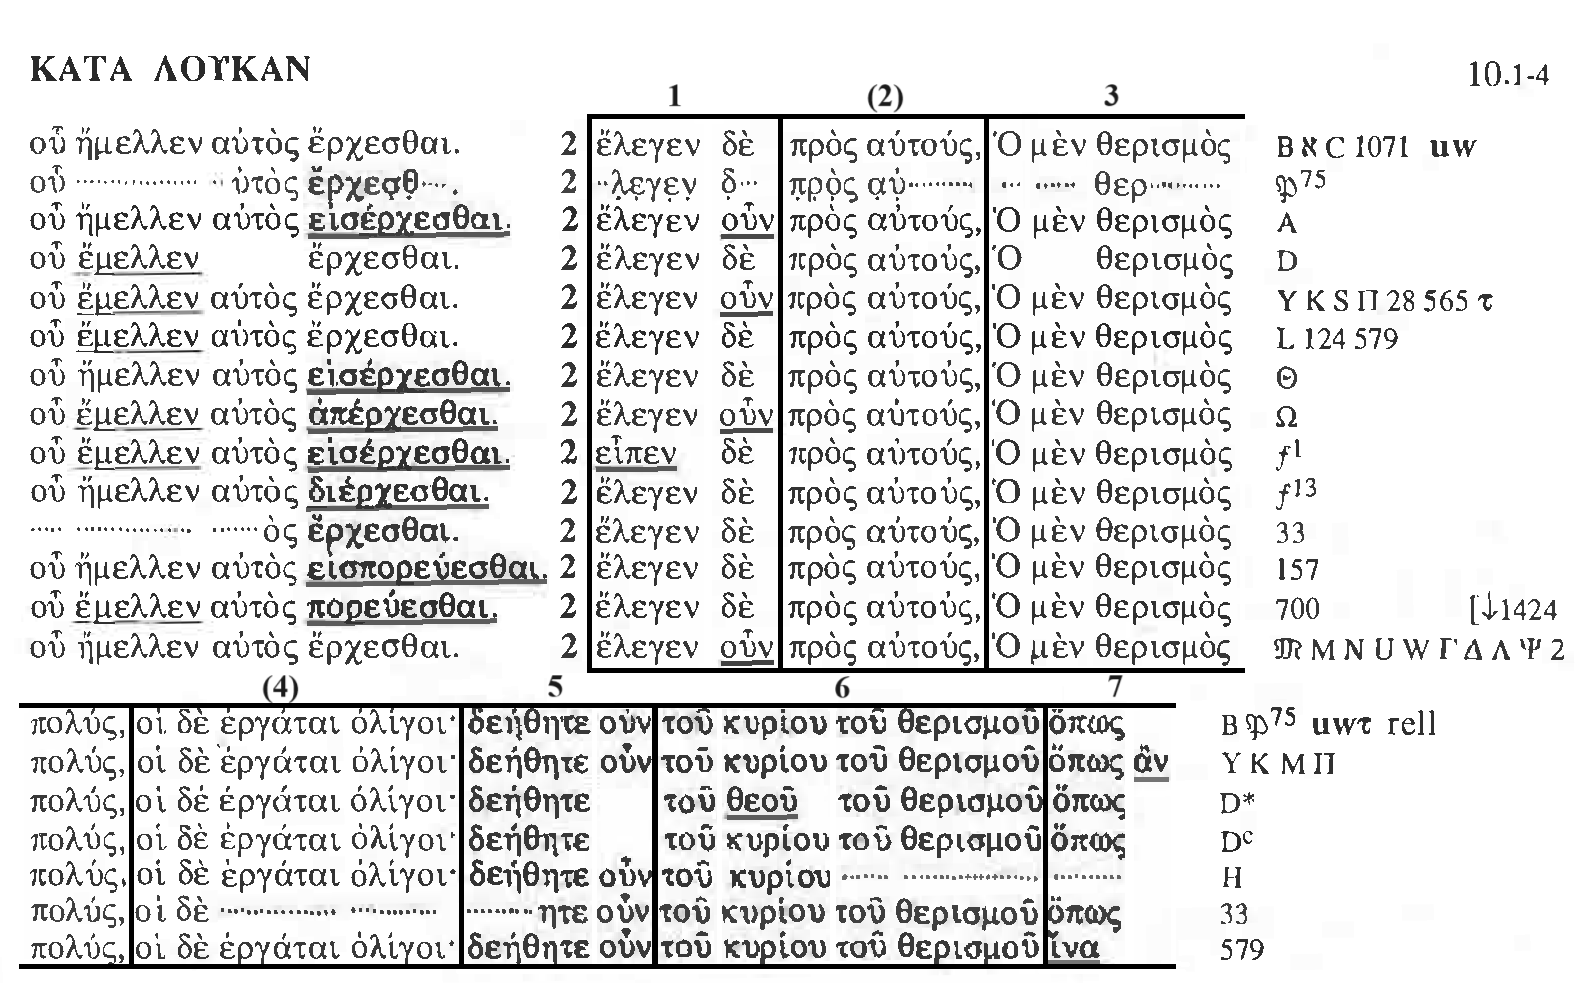
\includegraphics[width=0.75\textwidth]{../img/swanson-luke-10-2-variation-units.png}
		\end{center}
		\footnotesize Collation of Luke 10:2 with variation units numbered above text \parencite[183]{Swanson.Luke}
	\end{frame}
	\begin{frame}
		\begin{itemize}
			\item Analogous to a DNA sequence alignment
		\end{itemize}
		\begin{center}
			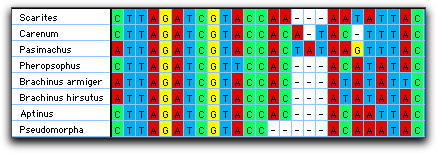
\includegraphics[scale=0.5]{../img/sequence-alignment.jpg}
		\end{center}
		\begin{itemize}
			\item Rows: \emph{taxa} = witnesses
			\item Columns: \emph{sites} = variation units
			\item Cells: \emph{states} = variant readings (including omissions)
			\begin{itemize}
				\item Lacunae and uncertain retroversions correspond to fully or partially \emph{ambiguous states}
			\end{itemize}
		\end{itemize}
	\end{frame}
	\subsection{Witnesses}
	\begin{frame}
		\begin{itemize}
			\item At the most basic level, a \emph{witness} is just a sequence of readings, a row in the collation
		\end{itemize}
		\begin{center}
			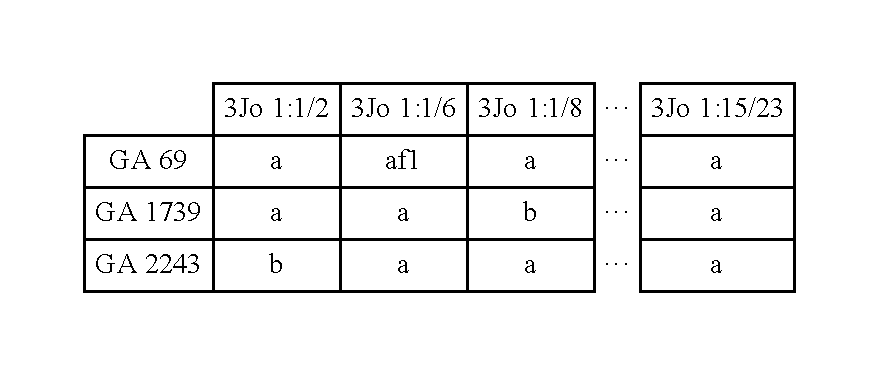
\includegraphics[scale=0.5]{../img/witnesses.pdf}
		\end{center}
		\begin{itemize}
			\item Paratextual features can be encoded in the same way
			\item In more complex phylogenetic approaches, age can also be incorporated
		\end{itemize}
	\end{frame}
	\section{Phylogenetics}
	\sectionframe
	\subsection{Fundamentals}
	\begin{frame}
		\begin{center}
			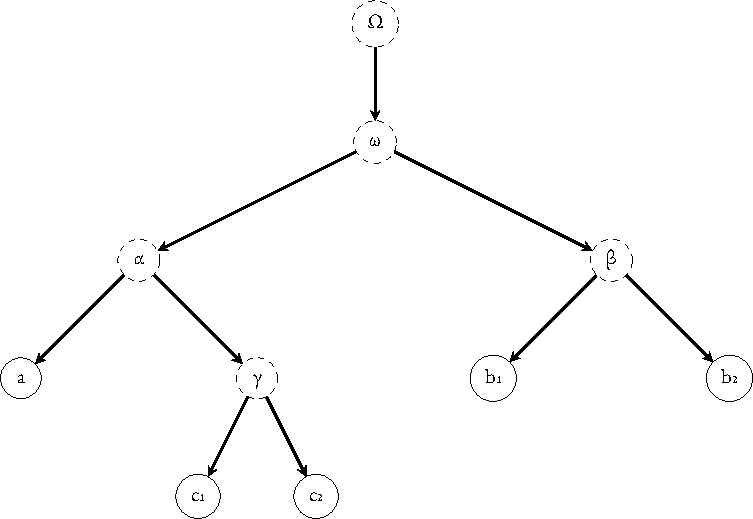
\includegraphics[scale=0.5]{../img/gene-tree-rooted-site-1.pdf}
		\end{center}
		\begin{itemize}
			\item A \emph{stemma} is a \textquote{family tree} modeling the transmission of the text
			\item The \emph{leaves} (solid circles) correspond to extant witnesses
			\item The \emph{hyparchetypes} (dashed circles) are hypothetical (now-lost) ancestors, reconstructed from their descendents along the branches
			\item The \emph{archetype} ({\renewfontfamily\greekfont[Script=Greek]{EB Garamond}\textgreek{ω}}) is the earliest reconstructible text
			\item The \emph{root} ({\renewfontfamily\greekfont[Script=Greek]{EB Garamond}\textgreek{Ω}}) represents the authorial text
		\end{itemize}
	\end{frame}
	\begin{frame}
		\begin{tabular}{p{0.4\textwidth} @{\hskip 0.1\textwidth} p{0.5\textwidth}}
			\vspace{0pt}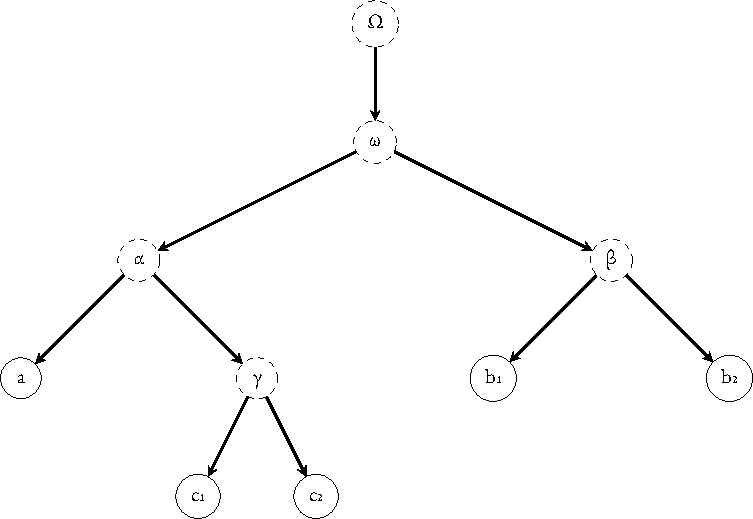
\includegraphics[scale=0.4]{../img/gene-tree-rooted-site-1.pdf} & \vspace{0pt}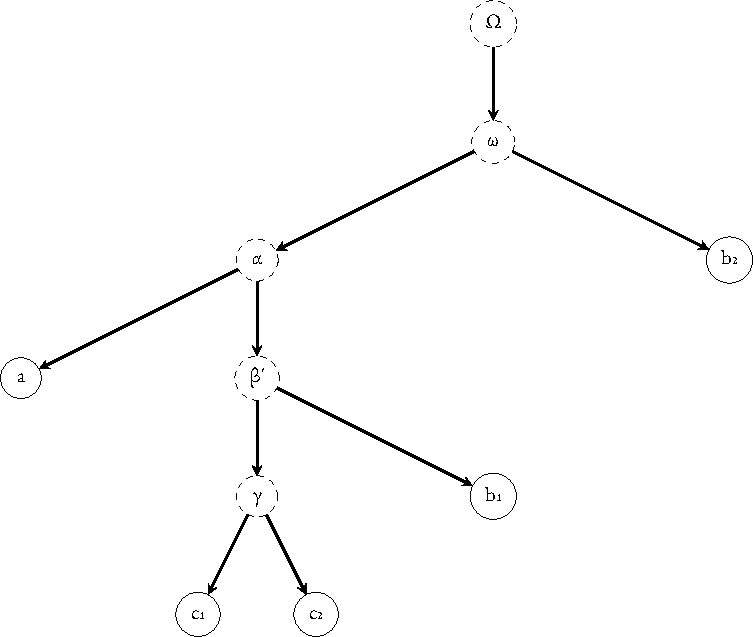
\includegraphics[scale=0.4]{../img/gene-tree-rooted-site-2.pdf}
		\end{tabular}
		\begin{itemize}
			\item A stemma represents a hypothesis about transmission history
			\item The goal is to determine which hypothesis (or hypotheses) best explain the extant data
			\item To do this, we need a numerical metric for the fitness of a given stemma
		\end{itemize}
	\end{frame}
	\subsection{Parsimony}
	\begin{frame}
		\begin{itemize}
			\item One such metric is \emph{parsimony}
			\item Cost = smallest number of changed readings along the branches of the stemma
			\item Motivated by Ockham's Razor
			\item Given a candidate stemma, we calculate its cost for each variation unit independently and add up the results
			\item We calculate it starting at the bottom of the stemma and working our way up
		\end{itemize}
		\begin{center}
			\setmainfont[Ligatures=Common]{EB Garamond}
			\renewfontfamily\greekfont[Script=Greek]{EB Garamond}
			\begin{tabular}{|l|l|}
				\hline
				Witness & Reading\\
				\hline
				\hline
				a & {\color{red}\textgreek{χριστου ιησου}}\\
				\hline
				b\textsubscript{1} & {\color{blue}\textgreek{ιησου χριστου}}\\
				\hline
				b\textsubscript{2} & {\color{blue}\textgreek{ιησου χριστου}}\\
				\hline
				c\textsubscript{1} & {\color{darkgreen}\textgreek{χριστου}}\\
				\hline
				c\textsubscript{2} & {\color{red}\textgreek{χριστου ιησου}}\\
				\hline
			\end{tabular}
		\end{center}
	\end{frame}
	\begin{frame}
		\begin{center}
			Cost for stemma 1: \only<1>{\phantom{\textbf{2}}}\only<2-3>{\textbf{2}}\\
			\vspace{\baselineskip}
			\only<1>{
				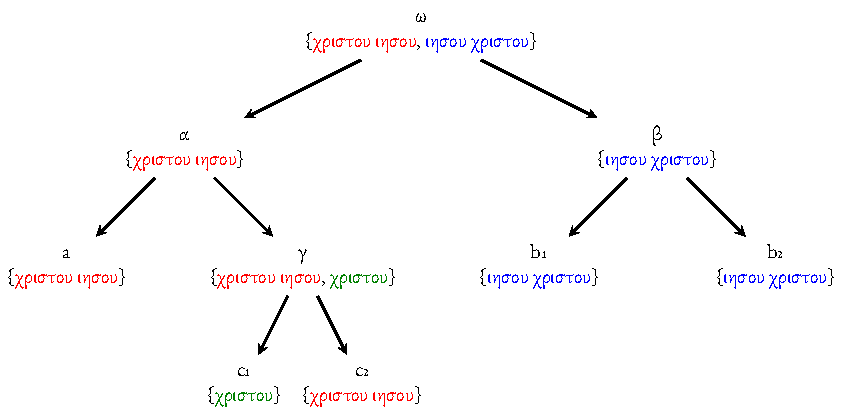
\includegraphics[scale=0.75]{../img/gene-tree-unrooted-forward-topology-1.pdf}
			}%
			\only<2>{
				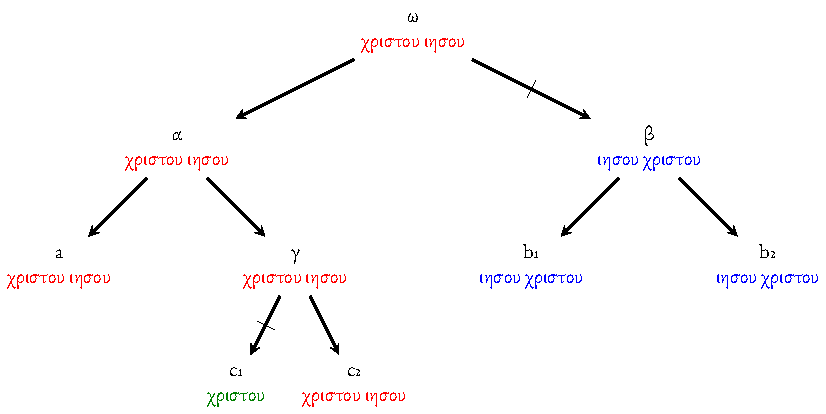
\includegraphics[scale=0.75]{../img/gene-tree-unrooted-backward-topology-1-option-1.pdf}
			}%
			\only<3>{
				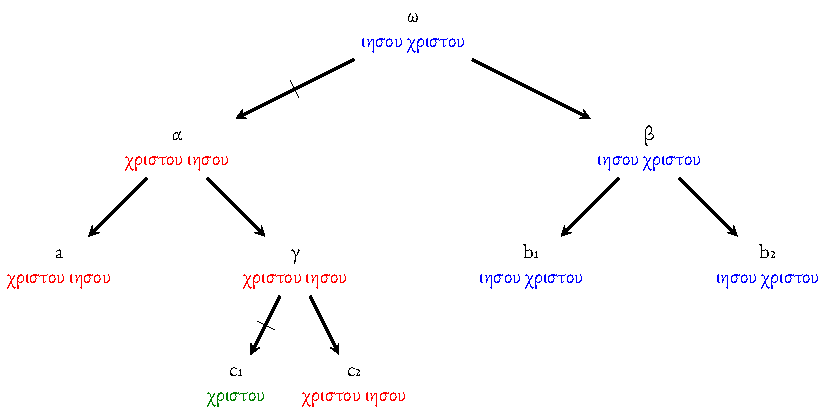
\includegraphics[scale=0.75]{../img/gene-tree-unrooted-backward-topology-1-option-2.pdf}
			}
		\end{center}
	\end{frame}
	\begin{frame}
		\begin{center}
			Cost for stemma 2: \only<1>{\phantom{\textbf{3}}}\only<2-3>{\textbf{3}}\\
			\vspace{\baselineskip}
			\only<1>{
				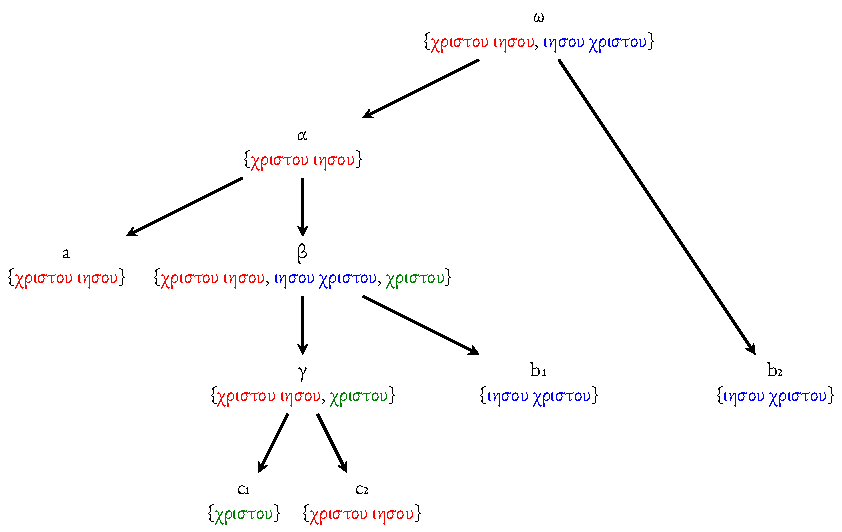
\includegraphics[scale=0.75]{../img/gene-tree-unrooted-forward-topology-2.pdf}
			}%
			\only<2>{
				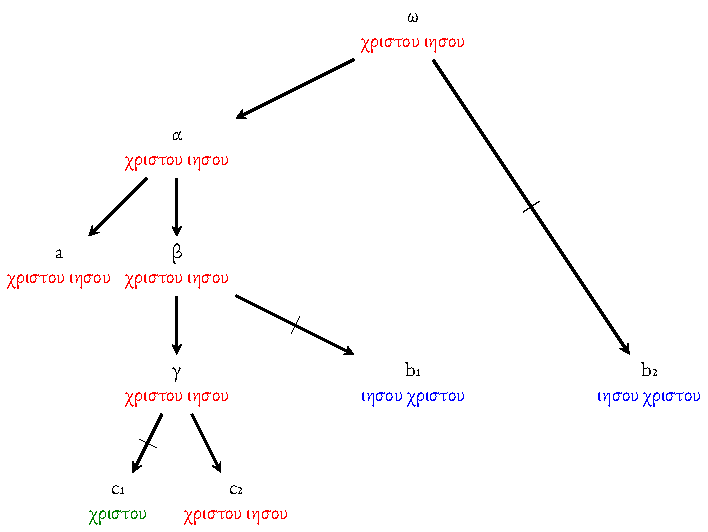
\includegraphics[scale=0.75]{../img/gene-tree-unrooted-backward-topology-2-option-1.pdf}
			}%
			\only<3>{
				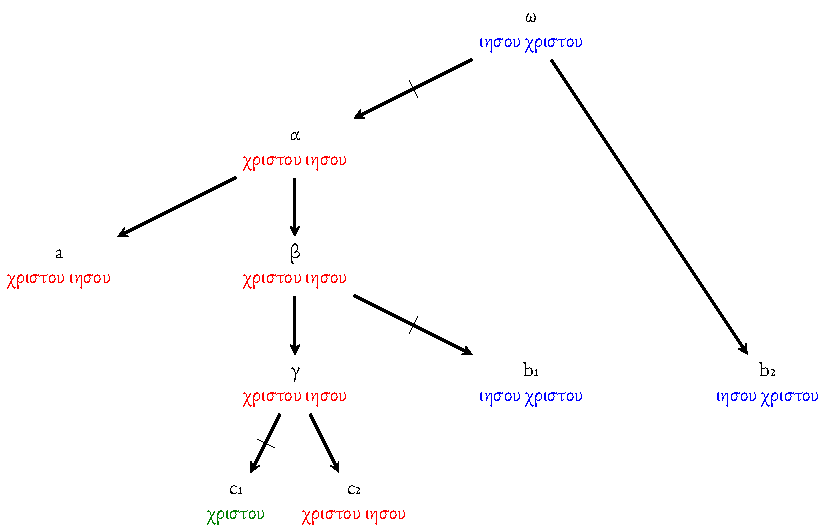
\includegraphics[scale=0.75]{../img/gene-tree-unrooted-backward-topology-2-option-2.pdf}
			}
		\end{center}
	\end{frame}
	\begin{frame}
		\begin{columns}[T]
			\begin{column}{0.45\textwidth}
				\begin{itemize}
					\item Minimum number of changes is the same regardless of what the archetype reads
					\item A stemma's cost \emph{does not depend on where its root is}
					\item This means the computer can calculate the costs of stemmata without knowledge about the root, and we can postpone the assessment of internal evidence of readings to the end, when we want to determine where the root of the tradition is
					\item The traditional approach for computer-assisted stemmatics
				\end{itemize}
			\end{column}
			\begin{column}{0.5\textwidth}
				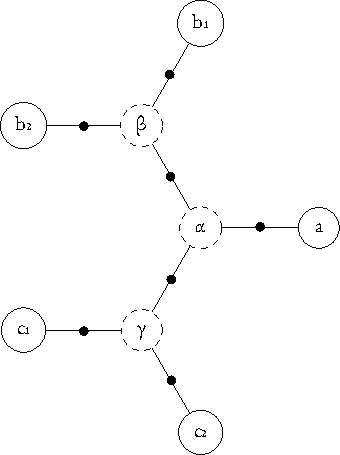
\includegraphics[scale=1]{../img/stemma-unrooted-potential-roots.pdf}
			\end{column}
		\end{columns}
	\end{frame}
%	\begin{frame}
%		\begin{itemize}
%			\item To get the total score of a stemma, add up its scores at each variation unit
%		\end{itemize}
%		\begin{columns}
%			\begin{column}{0.45\textwidth}
%				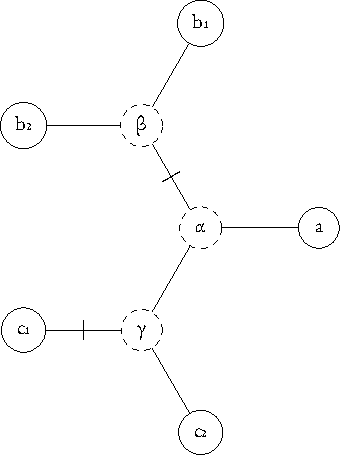
\includegraphics[scale=0.4]{../img/gene-tree-unrooted-site-1.pdf}\hfill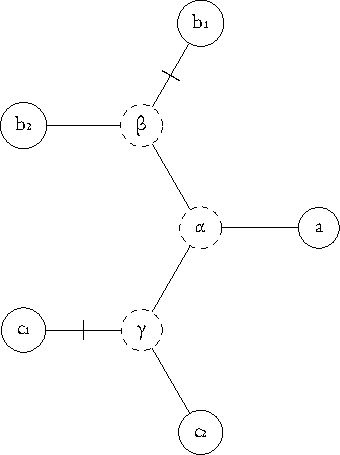
\includegraphics[scale=0.4]{../img/gene-tree-unrooted-site-2.pdf}\\
%				\vspace{2\baselineskip}
%				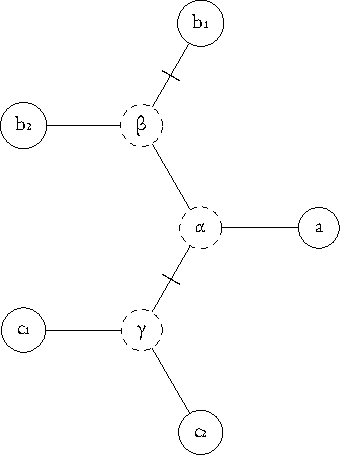
\includegraphics[scale=0.4]{../img/gene-tree-unrooted-site-3.pdf}\hfill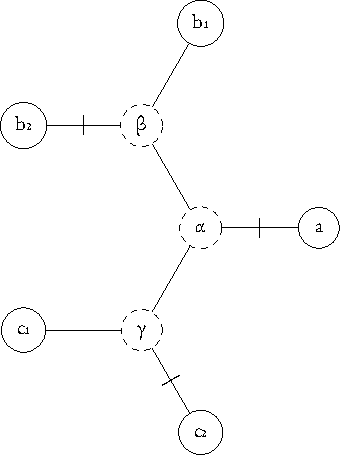
\includegraphics[scale=0.4]{../img/gene-tree-unrooted-site-4.pdf}
%			\end{column}
%			\begin{column}{0.1\textwidth}
%				\LARGE$\Rightarrow$
%			\end{column}
%			\begin{column}{0.45\textwidth}
%				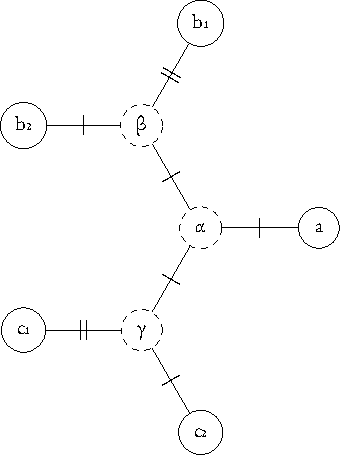
\includegraphics[scale=0.8]{../img/stemma-unrooted.pdf}
%			\end{column}
%		\end{columns}
%	\end{frame}
	\subsection{Extensions}
	\begin{frame}
		\begin{itemize}
			\item But we may want to incorporate internal evidence up front:
			\begin{itemize}
				\item Separation of concerns between \emph{intrinsic probabilities} (\textquote{what would the author write?}) and \emph{transcriptional probabilities} (\textquote{how would later scribes/readers change it?})
				\item Intrinsic probabilities can affect the backward pass
				\item Transcriptionally, some changes are more likely than others or irreversible
			\end{itemize}
			\item We can extend the approach to incorporate this evidence, but the stemma costs will now depend on where the root of the tradition is located
		\end{itemize}
		\begin{center}
			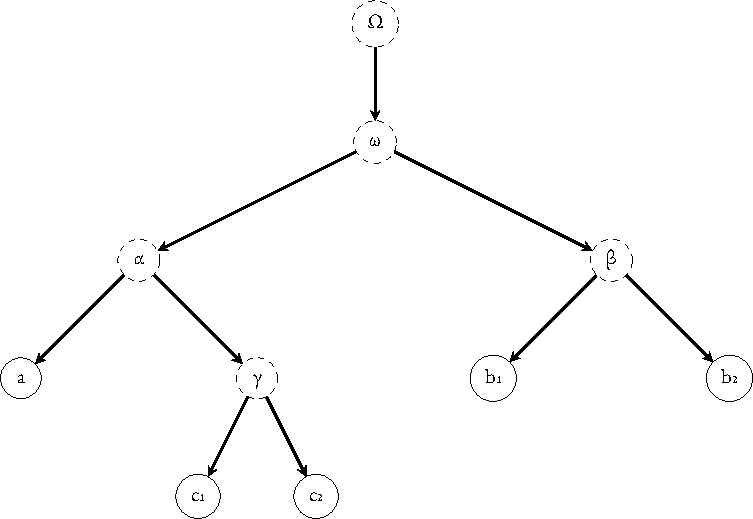
\includegraphics[scale=0.5]{../img/gene-tree-rooted-site-1.pdf}
		\end{center}
	\end{frame}
	\begin{frame}
		\begin{center}
			Cost for stemma: \only<1>{\phantom{\textbf{3}}}\only<2-4>{\textbf{3}}\\
			\vspace{\baselineskip}
			\only<1>{
				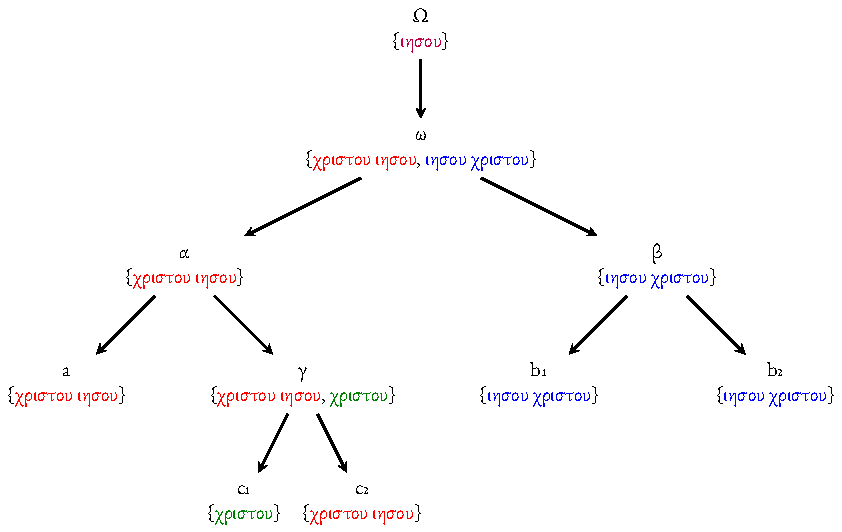
\includegraphics[scale=0.75]{../img/gene-tree-rooted-forward.pdf}
			}%
			\only<2>{
				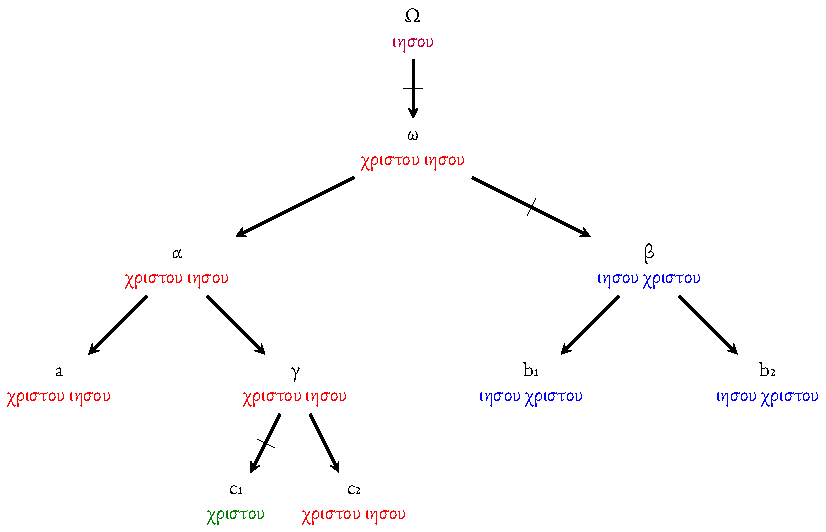
\includegraphics[scale=0.75]{../img/gene-tree-rooted-backward-option-1.pdf}
			}%
			\only<3>{
				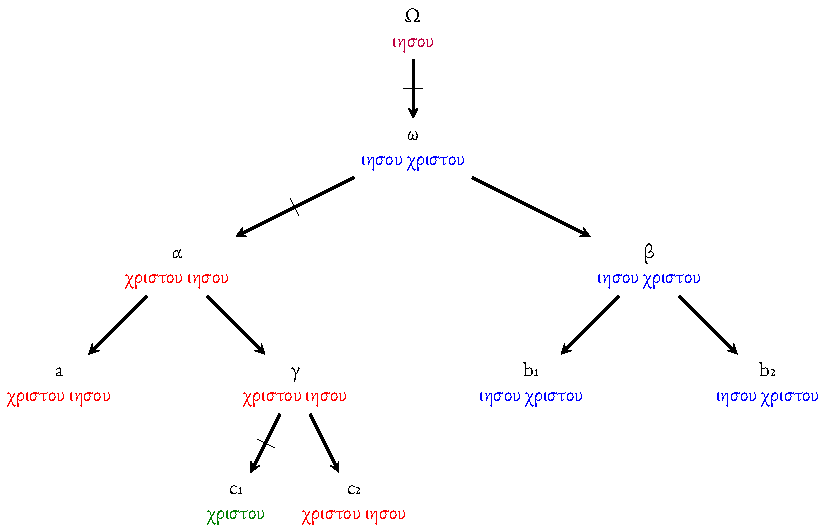
\includegraphics[scale=0.75]{../img/gene-tree-rooted-backward-option-2.pdf}
			}%
			\only<4>{
				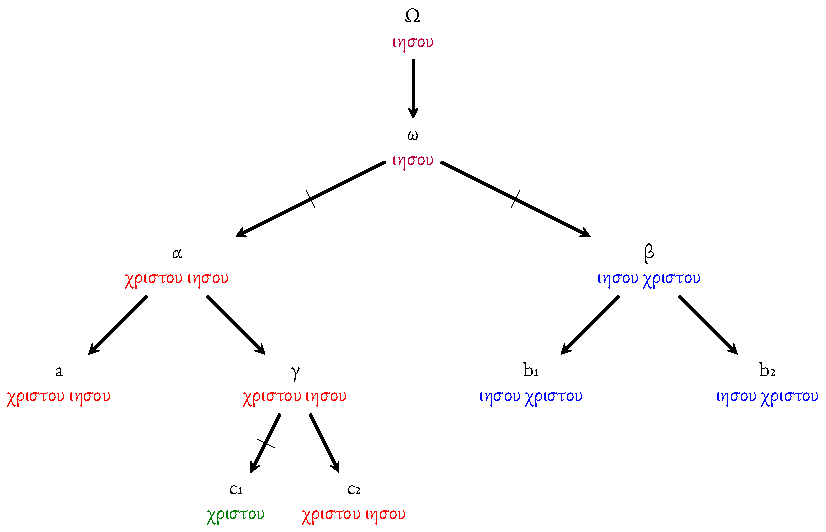
\includegraphics[scale=0.75]{../img/gene-tree-rooted-backward-option-3.pdf}
			}
		\end{center}
	\end{frame}
	\begin{frame}
		\begin{itemize}
			\item We can likewise assign weighted costs to different transitions between readings using a \emph{cost matrix}
			\item A model of the average scribe's behavior
		\end{itemize}
		\begin{center}
			\begin{columns}[T]
				\begin{column}{0.3\textwidth}
					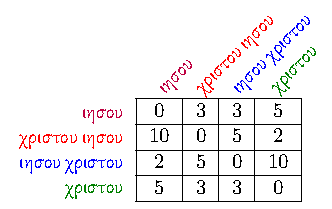
\includegraphics[scale=0.6667]{../img/sankoff-cost-matrix.pdf}
				\end{column}
				\begin{column}{0.65\textwidth}
					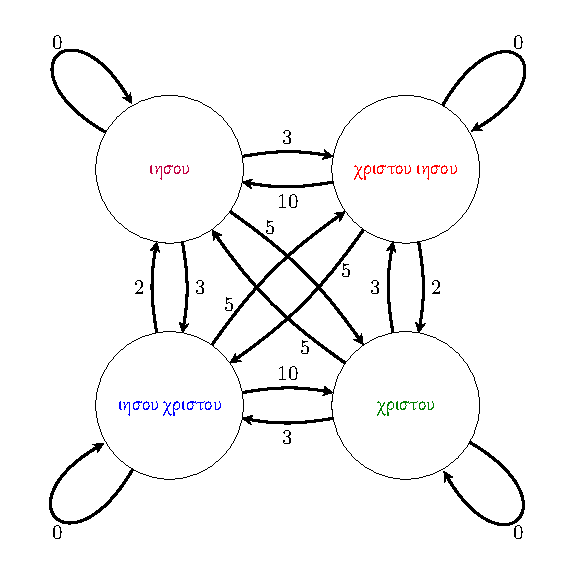
\includegraphics[scale=0.6667]{../img/sankoff-cost-graph.pdf}
				\end{column}
			\end{columns}
		\end{center}
	\end{frame}
	\begin{frame}
		\begin{itemize}
			\item For each hypearchetype, compute the current minimum cost for each reading it could have based on the minimum costs of its children
			\item For example, the minimum cost of {\renewfontfamily\greekfont[Script=Greek]{EB Garamond}\textgreek{γ}} reading \textgreek{ιησου} is the cost of the transition from \textgreek{ιησου} to \textgreek{χριστου} (in {\setmainfont{EB Garamond}c\textsubscript{1}}) plus the cost of the transition from \textgreek{ιησου} to \textgreek{χριστου ιησου} (in {\setmainfont{EB Garamond}c\textsubscript{2}}): $(5+0) + (3+0) = \mathbf{8}$
		\end{itemize}
		\vspace{0.025\baselineskip}
		\begin{center}
			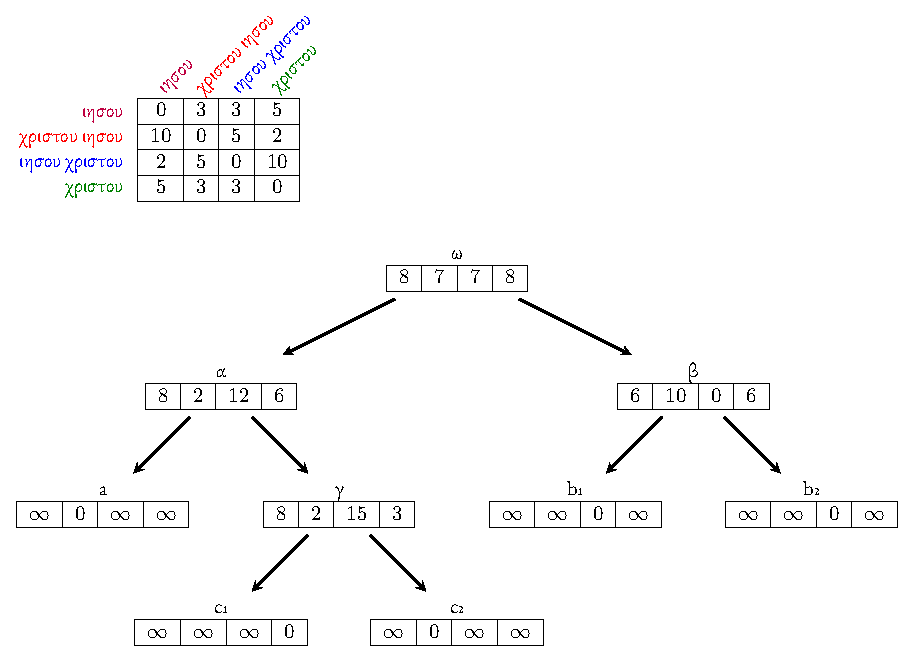
\includegraphics[scale=0.5]{../img/gene-tree-unrooted-sankoff.pdf}
		\end{center}
	\end{frame}
	\begin{frame}
		\begin{itemize}
			\item For {\renewfontfamily\greekfont[Script=Greek]{EB Garamond}\textgreek{α}} reading \textgreek{ιησου}, it is $3+0$ (for the transition to \textgreek{χριστου ιησου} in {\setmainfont{EB Garamond}a}) plus $\min(0+8, 3+2, 3+15, 5+3)$ $= \min(8, 5, 18, 8)$ $= 5$ (for transitions to any of the readings in {\renewfontfamily\greekfont[Script=Greek]{EB Garamond}\textgreek{γ}}) $\Rightarrow \mathbf{8}$
			\item Meanwhile, for {\renewfontfamily\greekfont[Script=Greek]{EB Garamond}\textgreek{α}} reading \textgreek{χριστου ιησου}, this is $(0+0)$ for  {\setmainfont{EB Garamond}a} plus $\min(10+8, 0+2, 5+15, 2+3) = \min(18,2,20,5) = 2$ for {\renewfontfamily\greekfont[Script=Greek]{EB Garamond}\textgreek{γ}} $\Rightarrow \mathbf{2}$
		\end{itemize}
		\begin{center}
			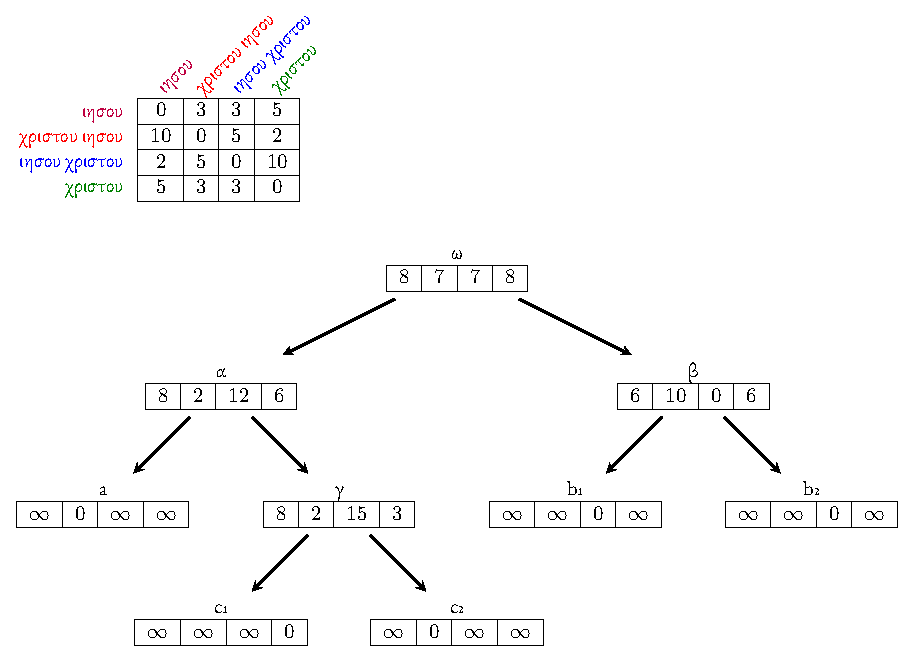
\includegraphics[scale=0.5]{../img/gene-tree-unrooted-sankoff.pdf}
		\end{center}
	\end{frame}
	\begin{frame}
		\begin{itemize}
			\item We can also incorporate intrinsic evidence
			\item If the root reading is \textgreek{ιησου}, then the minimum cost of the stemma is $\min(0+8, 3+7, 3+7, 5+8) = \min(8, 10, 10, 13) = \mathbf{8}$
			\item If the root reading is \textgreek{χριστου ιησου}, then the minimum cost is $\min(10+8, 0+7, 5+7, 2+8) = \min(18, 7, 12, 10) = \mathbf{7}$
		\end{itemize}
		\vspace{0.1\baselineskip}
		\begin{center}
			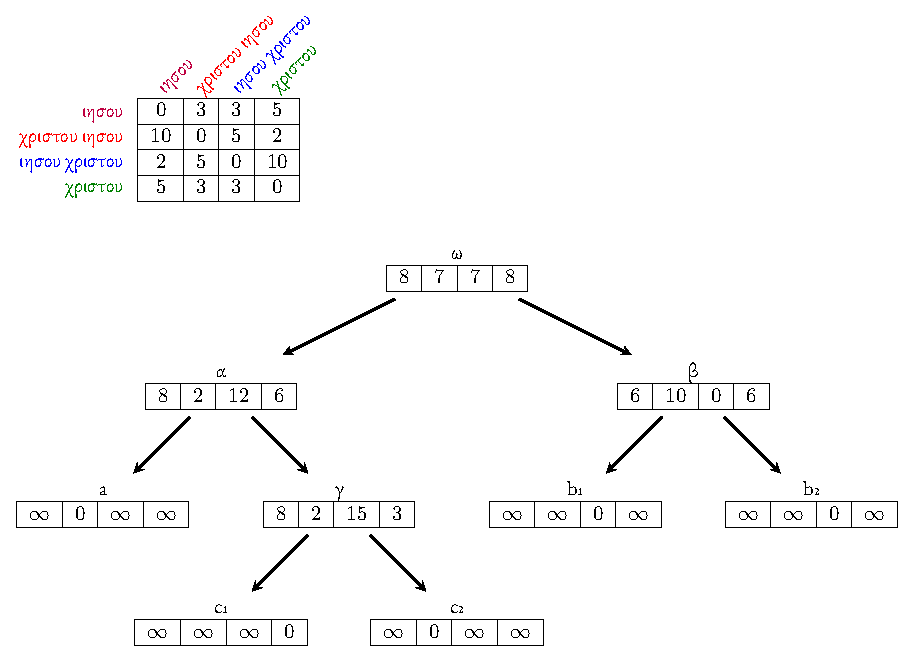
\includegraphics[scale=0.5]{../img/gene-tree-unrooted-sankoff.pdf}
		\end{center}
	\end{frame}
	\begin{frame}
		\begin{itemize}
			\item We can even use probabilities for intrinsic and transcriptional evidence
			\item Intrinsic probabilities = \emph{prior probabilities} at root
			\item Transcriptional probabilities = probabilities of copying the same reading or changing it to another reading, modeled as a \emph{Markov chain}
		\end{itemize}
		\begin{center}	
			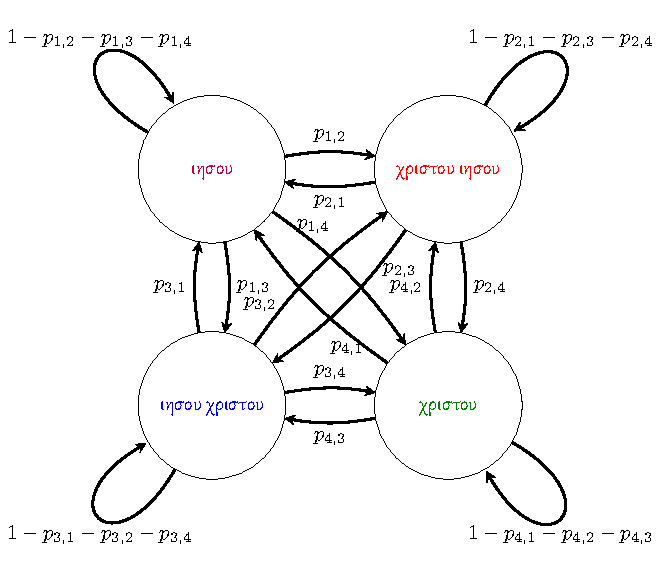
\includegraphics[scale=0.6667]{../img/markov-chain.pdf}
		\end{center}
	\end{frame}
	\begin{frame}
		\begin{itemize}
			\item In a probabilistic setting, we can incorporate and estimate other parameters of interest:
			\begin{itemize}
				\item Probabilities for classes of transitions between readings (scribal habits)
				\item Lengths of branches (how many copying events separated an ancestor from a descendent, and how error-prone were the scribes involved?)
				\item Dates of witnesses (using clock models)
				\item Measurements of how certain we can be about the best stemmata found in the process
			\end{itemize}
			\item More complex, but feasible with modern computers!
		\end{itemize}
		\begin{center}	
			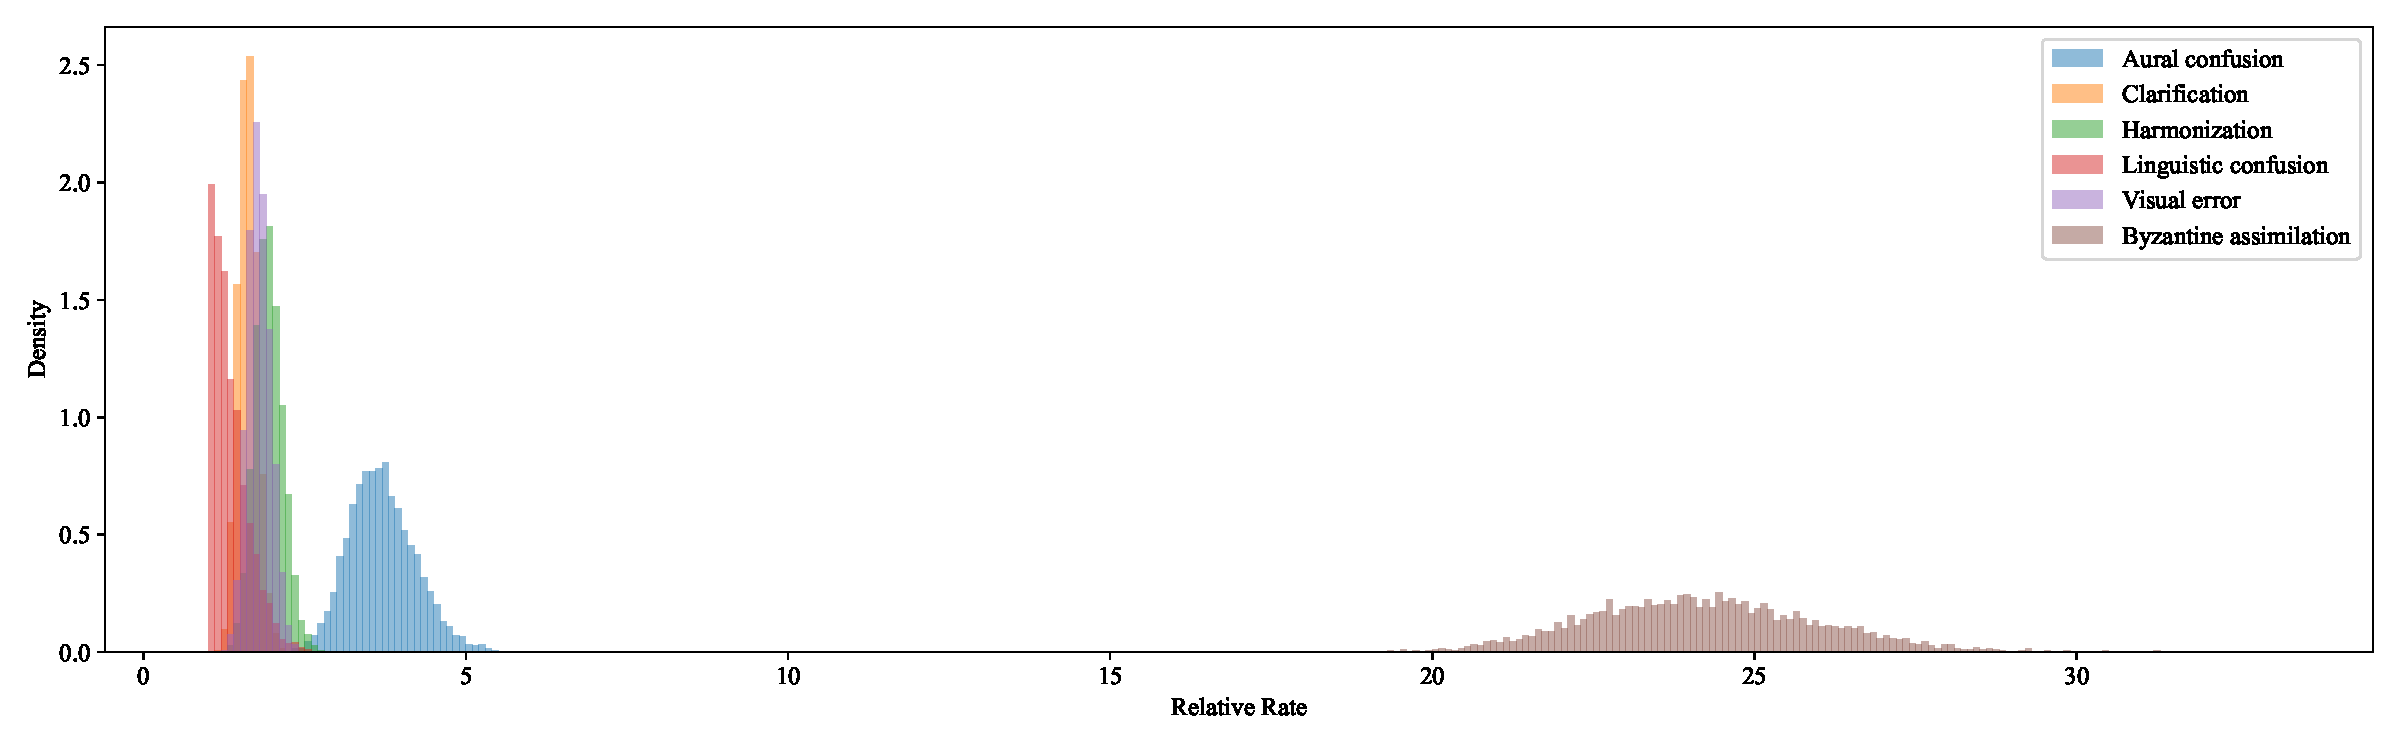
\includegraphics[scale=0.25]{../img/ecm-mark-local-rates.pdf}
		\end{center}
	\end{frame}
	\section{CBGM}
	\sectionframe
	\subsection{Fundamentals}
%	\begin{frame}
%		\begin{itemize}
%			\item Developed over thirty years by Gerd Mink, culminating in the latest updates to the \emph{Editio Critica Maior} (\emph{ECM})
%			\item Important reading:
%			\begin{itemize} 
%				\item \cite{Mink04}
%				\item \cite{Gurry17}
%				\item \cite{WG17}
%				\item \cite{Edmondson19}
%			\end{itemize}
%		\end{itemize}
%	\end{frame}
%	\begin{frame}
%		\begin{itemize}
%			\item \emph{Not} a way to make computers do textual criticism, but a way for them to help us refine our judgments
%			\item \emph{Not} a new methodology for evaluating variant readings, but a \textquote{meta-approach} to be used on top of existing methods
%		\end{itemize}
%	\end{frame}
	\begin{frame}
		\begin{itemize}
			\item Developed to solve \emph{contamination}, or mixture across branches of the textual tradition
		\end{itemize}
		\begin{center}
			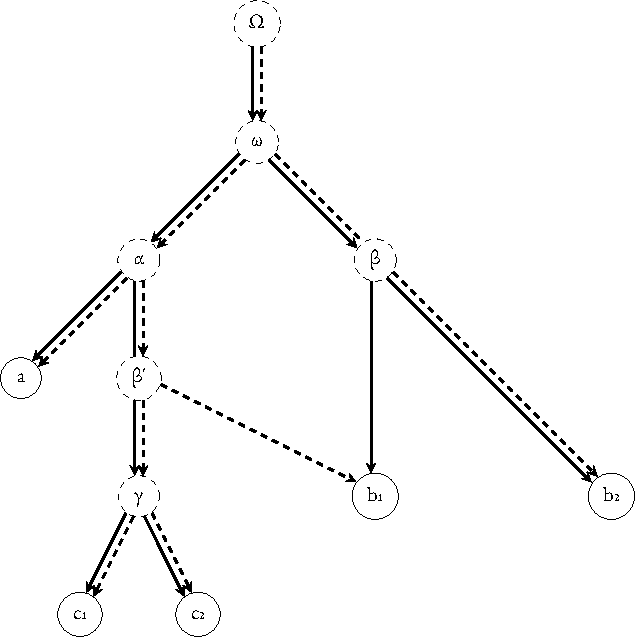
\includegraphics[scale=0.6667]{../img/stemma-rooted-contamination.pdf}
		\end{center}
	\end{frame}
	\begin{frame}
		\begin{itemize}
			\item Foundational principles:
			\begin{enumerate}
				\item Scribes typically copied their exemplars with fidelity.
				\item If a scribe introduced a variant, then it came from some other reading.
				\item Scribes typically used fewer sources rather than many.
				\item Scribes typically used closely related sources rather than distant ones.
			\end{enumerate}
			\item Witnesses are \emph{texts} (sequences of readings), minus the material baggage (date, provenance, etc.)
			\begin{itemize}
				\item \textquote{How texts relate} $\neq$ \textquote{How manuscripts relate}
			\end{itemize}
			\item \emph{No hypothetical ancestors} (except for the \emph{Ausgangstext} A)
			\begin{itemize}
				\item Contamination would (presumably) hinder their reconstruction
				\item Instead, we use extant witnesses as proxies for different states of the text
				\item This yields a much smaller and more manageable space of solutions compared to the space of all possible stemmata for a given set of witnesses
			\end{itemize}
		\end{itemize}
	\end{frame}
	\subsection{Local Stemmata}
	\begin{frame}
		\begin{itemize}
			\item The basic unit of comparison
			\item One for each variation unit
			\item A graphical representation of our judgments of readings
			\item Similar to cost graphs in function, but in principle, represents a judgment about what \emph{did} happen, not what \emph{could} happen
			\item Thus, no bidirectional edges or cycles like we have in cost graphs
		\end{itemize}
		\begin{columns}
			\begin{column}{0.45\textwidth}
				\begin{center}
					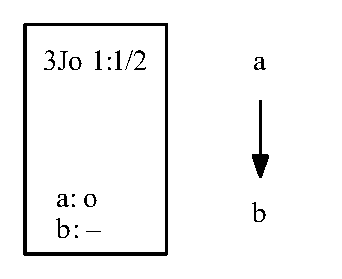
\includegraphics[scale=0.5]{../img/B25K1V1U2-local-stemma.pdf}
				\end{center}
			\end{column}
			\begin{column}{0.45\textwidth}
				\begin{center}
					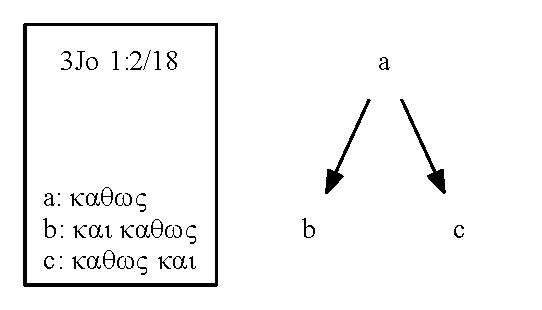
\includegraphics[scale=0.5]{../img/B25K1V2U18-local-stemma.pdf}
				\end{center}
			\end{column}
		\end{columns}
	\end{frame}
%	\begin{frame}
%		\begin{itemize}
%			\item Some are more complicated
%			\begin{itemize}
%				\item \emph{defective} readings (e.g., obvious misspellings)
%				\item \emph{orthographic} readings (e.g., regional differences)
%				\item \emph{split} attestations of the same reading (coincidental agreement)
%				\item \emph{ambiguous} readings
%			\end{itemize}
%			\item Some of these may be collapsed with other substantive readings
%			\begin{center}
%				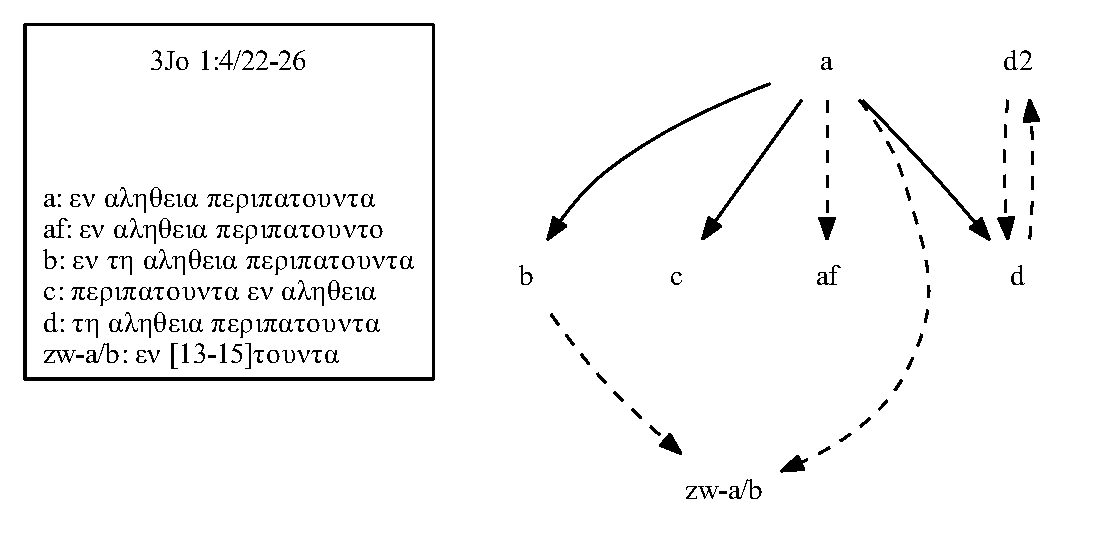
\includegraphics[scale=0.5]{../img/B25K1V4U22-26-local-stemma-ignore-defective-ignore-ambiguous-merge-splits.pdf}
%			\end{center}
%		\end{itemize}
%	\end{frame}
	\subsection{Genealogical Relationships}
	\begin{frame}
		\begin{itemize}
			\item The relationship of two witnesses is the overall pattern \emph{of the relationships of their readings} at all variation units where both are extant
		\end{itemize}
		\begin{center}
			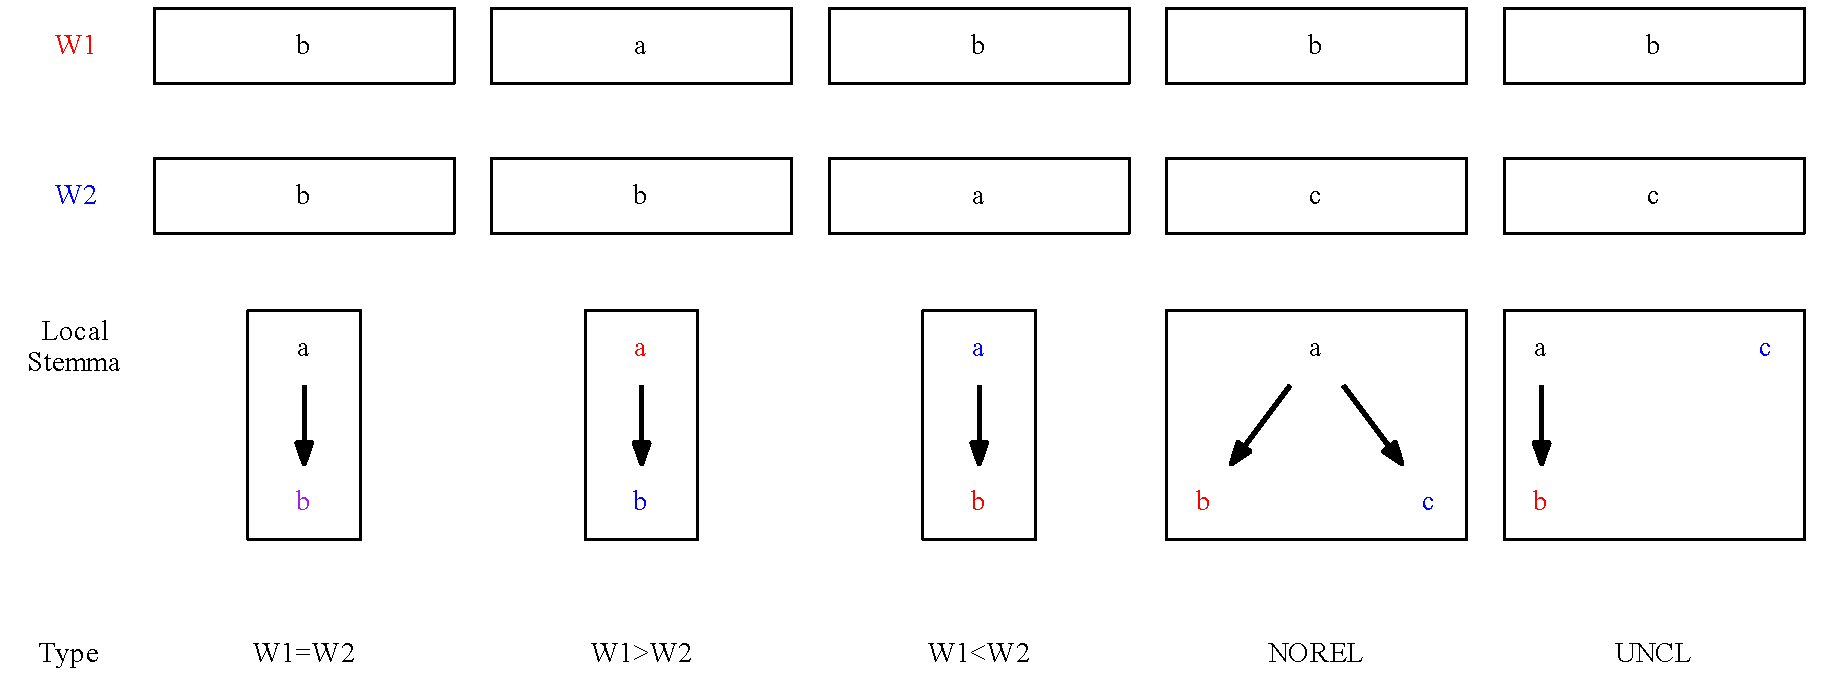
\includegraphics[width=\textwidth]{../img/genealogical-relationships.pdf}
		\end{center}
		\begin{itemize}
			\item The first three are the most important
		\end{itemize}
	\end{frame}
	\subsection{Potential Ancestors}
	\begin{frame}
		\begin{itemize}
			\item Potential ancestor = \textquote{more prior than posterior readings}
		\end{itemize}
		\begin{center}
			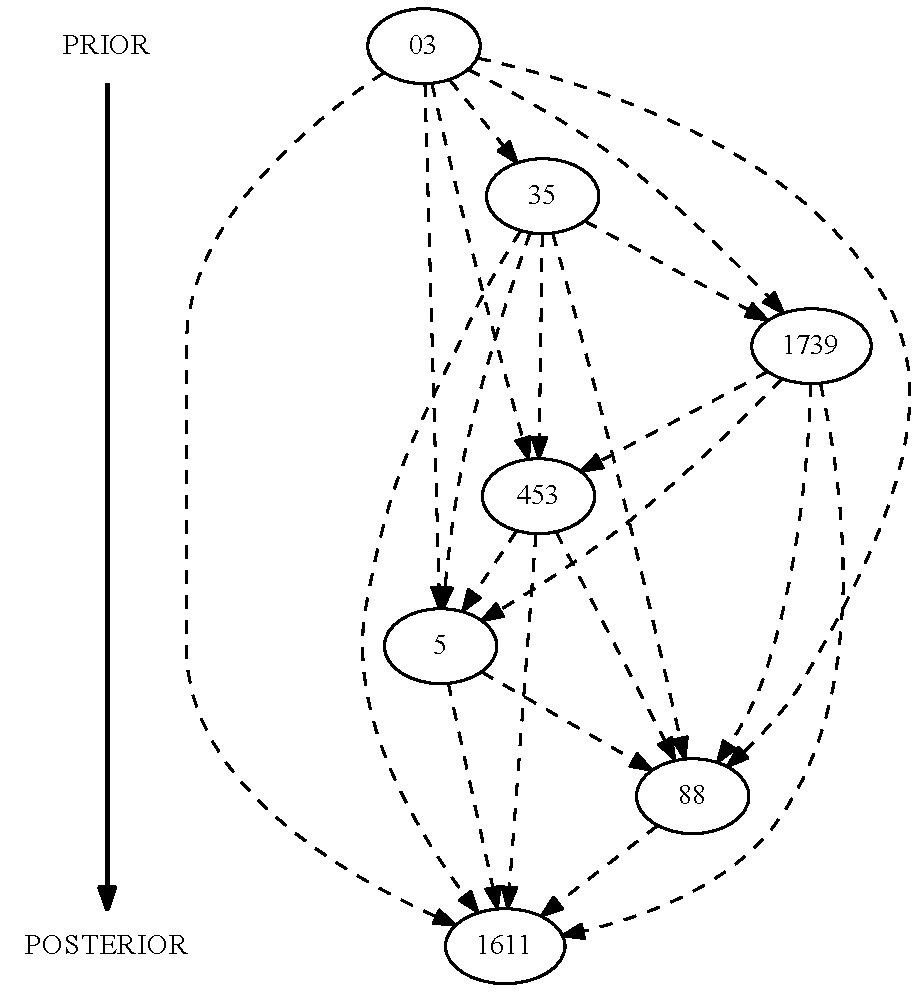
\includegraphics[scale=0.3333]{../img/potential-ancestors.pdf}
		\end{center}
	\end{frame}
	\subsection{Textual Flow}
%	\begin{frame}
%		\begin{columns}
%			\begin{column}{0.45\textwidth}
%				\begin{itemize}
%					\item \emph{Textual flow} is a useful tool for helping us revise our judgments in a local stemma
%					\item \emph{Not} a global stemma (our ultimate goal), but still important
%				\end{itemize}
%			\end{column}
%			\begin{column}{0.45\textwidth}
%				\begin{center}
%					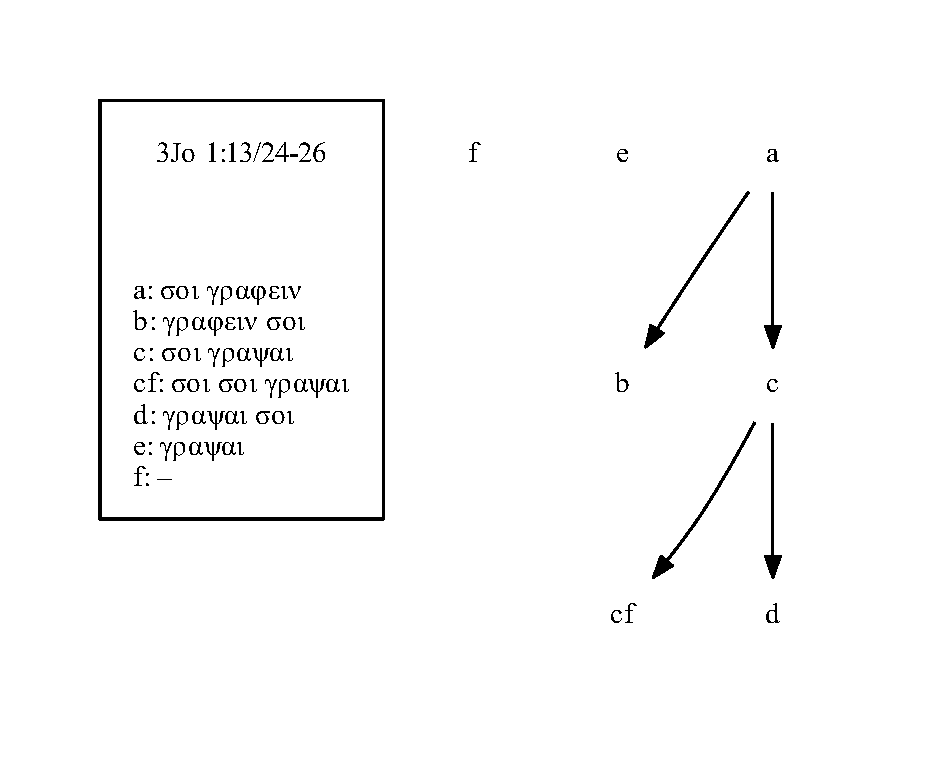
\includegraphics[width=\textwidth]{../img/B25K1V13U24-26-local-stemma-incomplete.pdf}
%				\end{center}
%			\end{column}
%		\end{columns}
%		\begin{center}
%			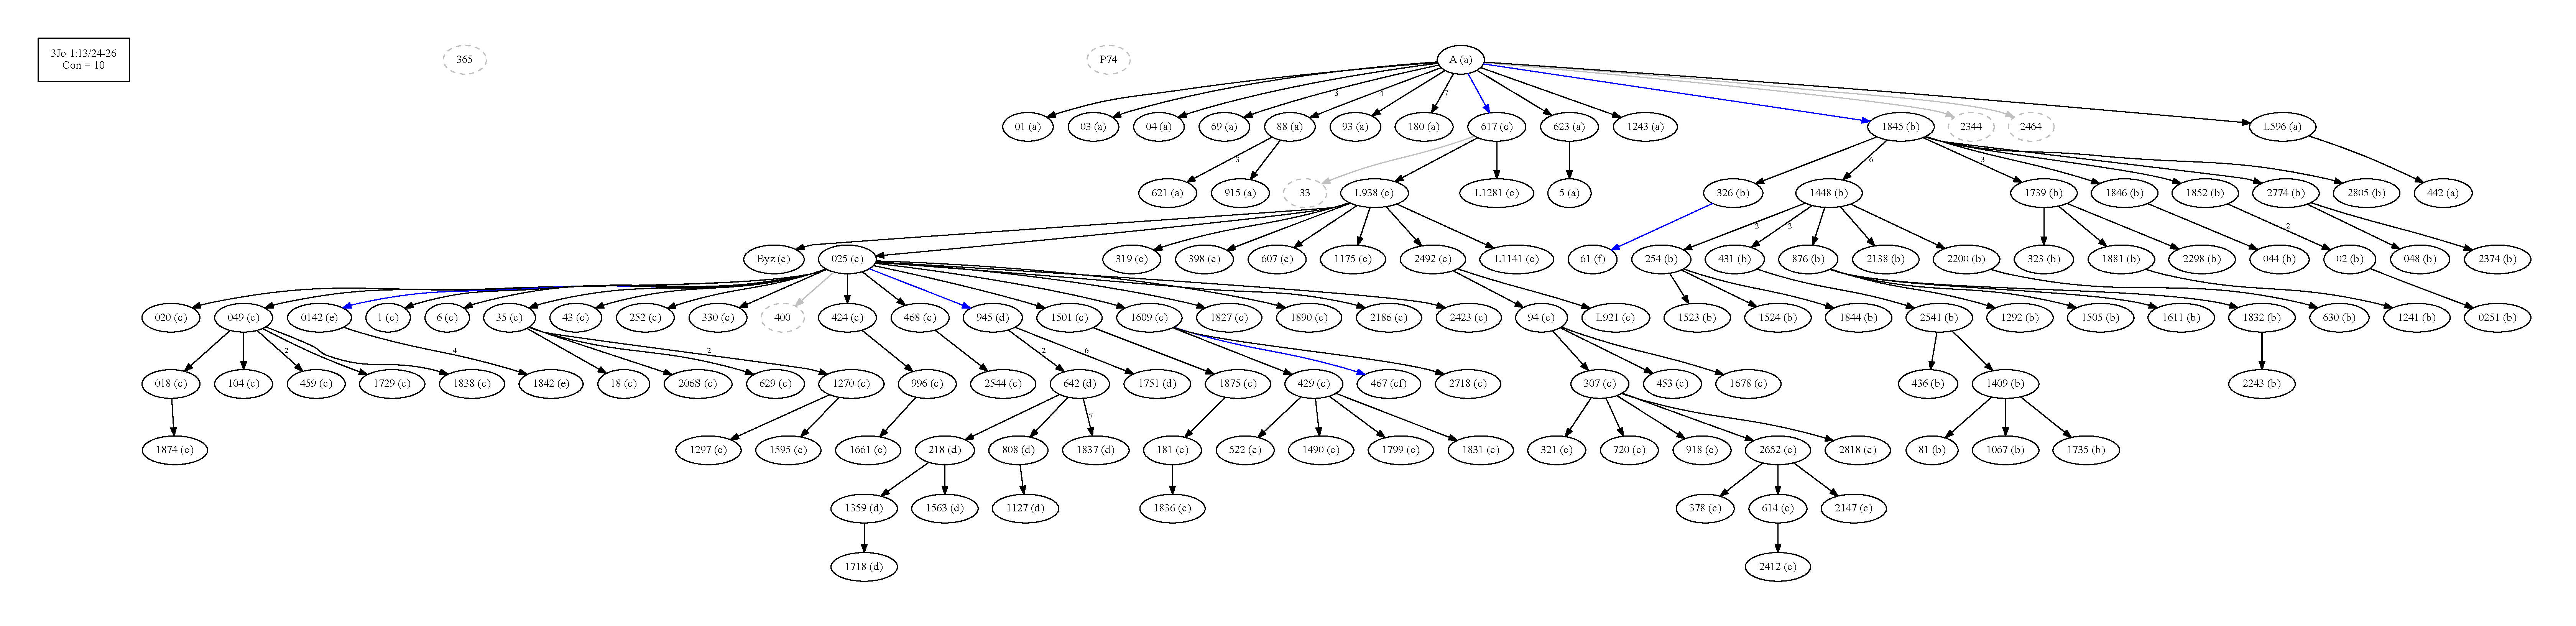
\includegraphics[width=\textwidth]{../img/B25K1V13U24-26-textual-flow.pdf}
%		\end{center}
%	\end{frame}
	\begin{frame}
		\begin{itemize}
			\item Textual flow diagram = a tree that relates each witness to its closest potential ancestor, with as few changes in reading as possible
			\item Similar to a most-parsimonious stemma for a specific variation unit
			\item We specify a \emph{connectivity limit} {\renewfontfamily\greekfont[Script=Greek]{EB Garamond}\textgreek{κ}} (i.e., a radius of \textquote{close-enough} neighbors)
			\item Then, for each witness:
			\begin{enumerate}
				\item List its potential ancestors, sorted from most agreement to least
				\item If one of the first {\renewfontfamily\greekfont[Script=Greek]{EB Garamond}\textgreek{κ}} has the same reading at this unit, then select it
				\item If not, then choose the first (non-lacunose) potential ancestor
			\end{enumerate}
			\item Core idea: use \emph{general relationships} between witnesses to find \emph{specific relationships} between readings, so local stemmata can be refined
		\end{itemize}
		\begin{center}
			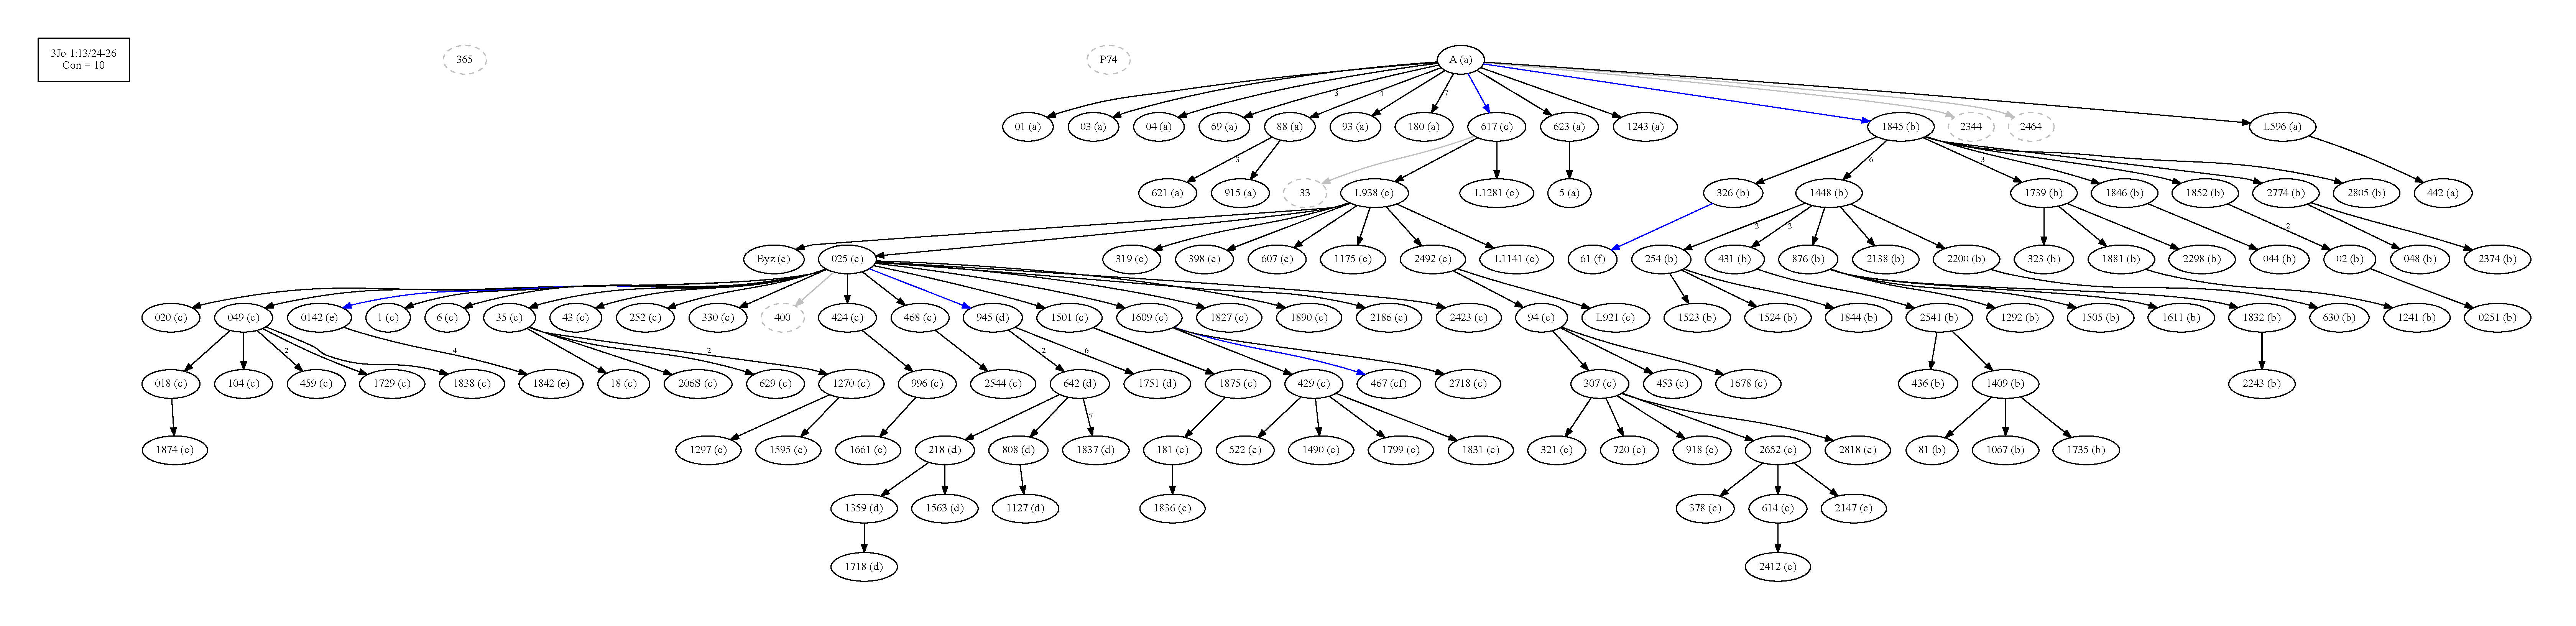
\includegraphics[width=\textwidth]{../img/B25K1V13U24-26-textual-flow.pdf}
		\end{center}
	\end{frame}
%	\begin{frame}
%		\begin{itemize}
%			\item Often, we just want to know the textual flow for witnesses with a specific reading
%		\end{itemize}
%		\begin{center}
%			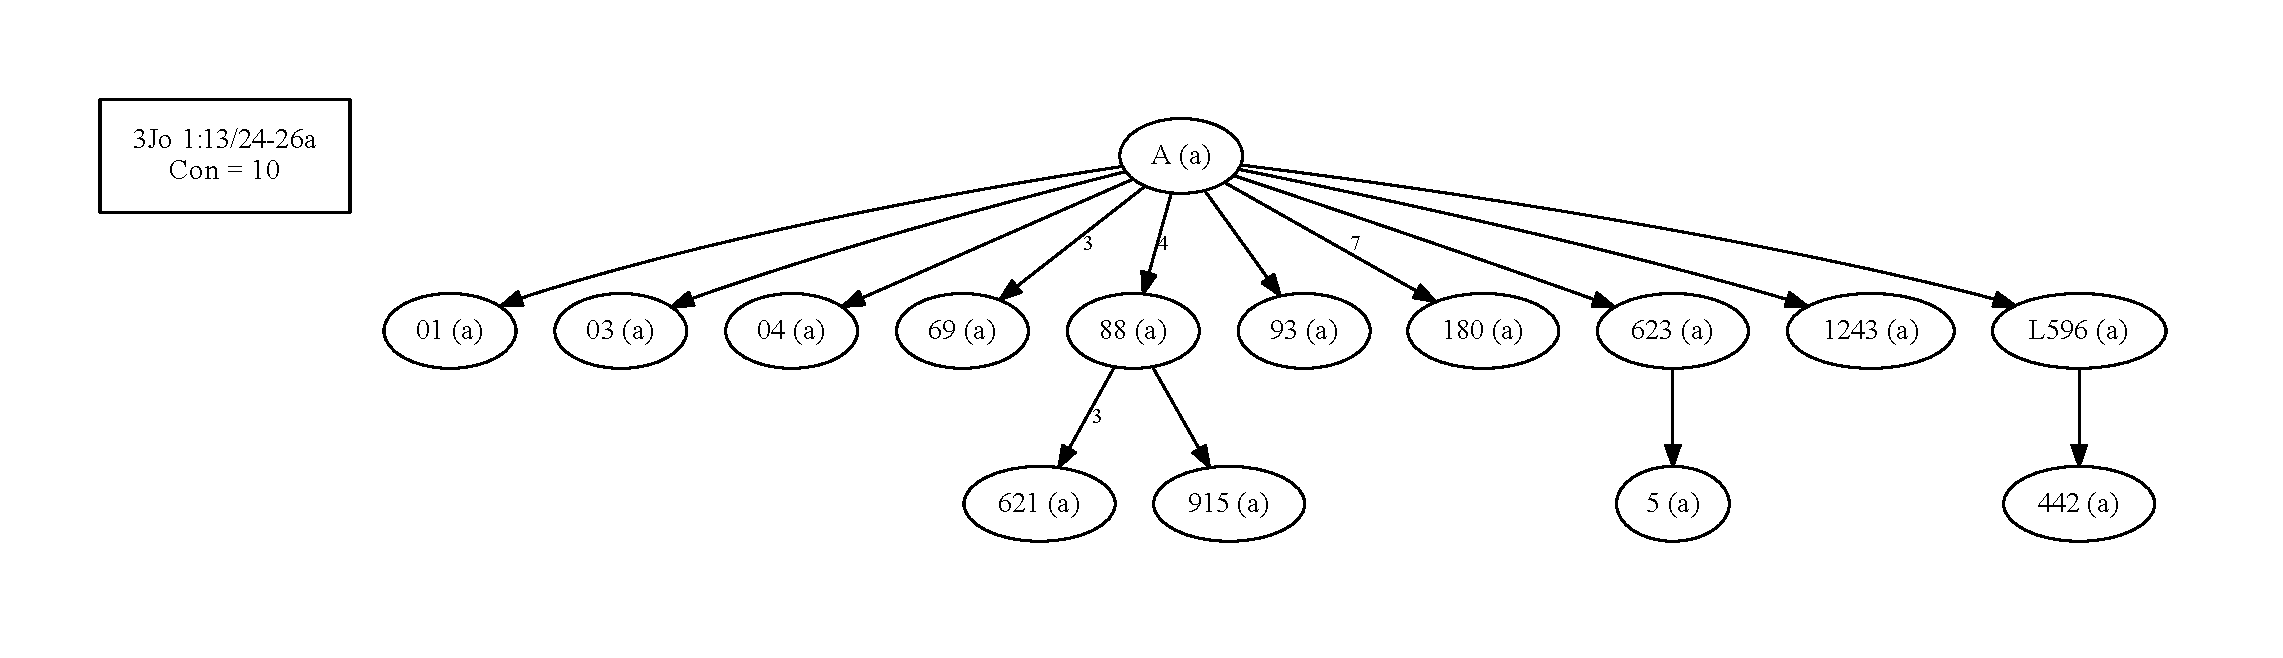
\includegraphics[width=\textwidth]{../img/B25K1V13U24-26Ra-coherence-attestations.pdf}
%		\end{center}
%		\begin{itemize}
%			\item (Numbers on edges represent the rank of the closest potential ancestor with the same reading, if it's not 1)
%		\end{itemize}
%	\end{frame}
%	\begin{frame}
%		\begin{itemize}
%			\item We can use it to evaluate alternate hypotheses about the initial text (A)
%		\end{itemize}
%		\begin{columns}
%			\begin{column}{0.45\textwidth}
%				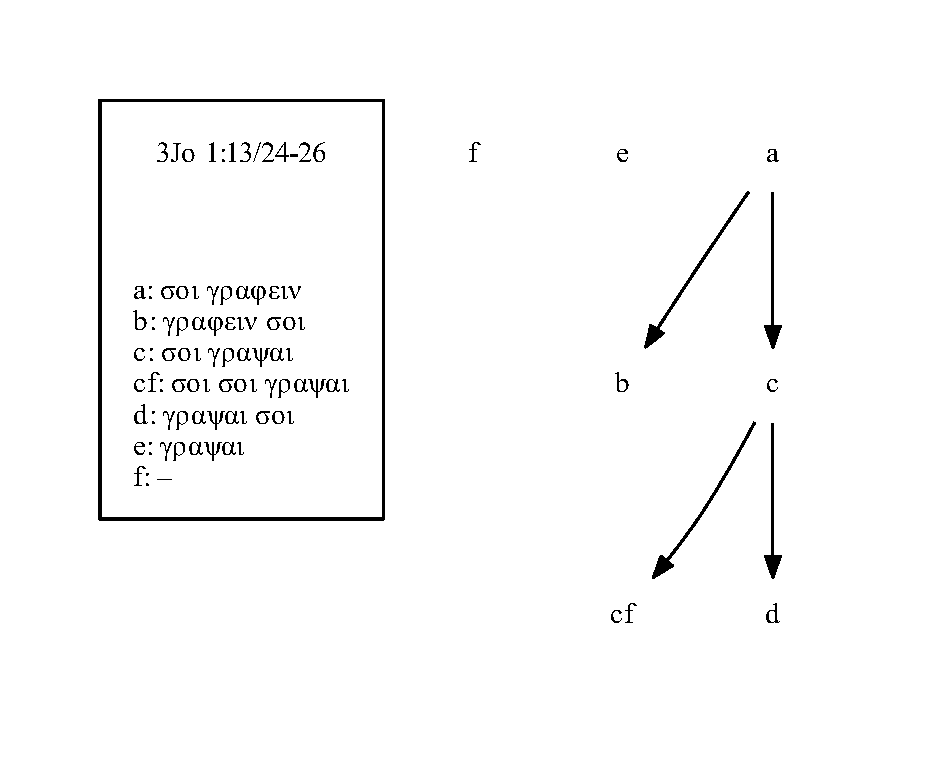
\includegraphics[width=\textwidth]{../img/B25K1V13U24-26-local-stemma-incomplete.pdf}
%			\end{column}
%			\begin{column}{0.45\textwidth}
%				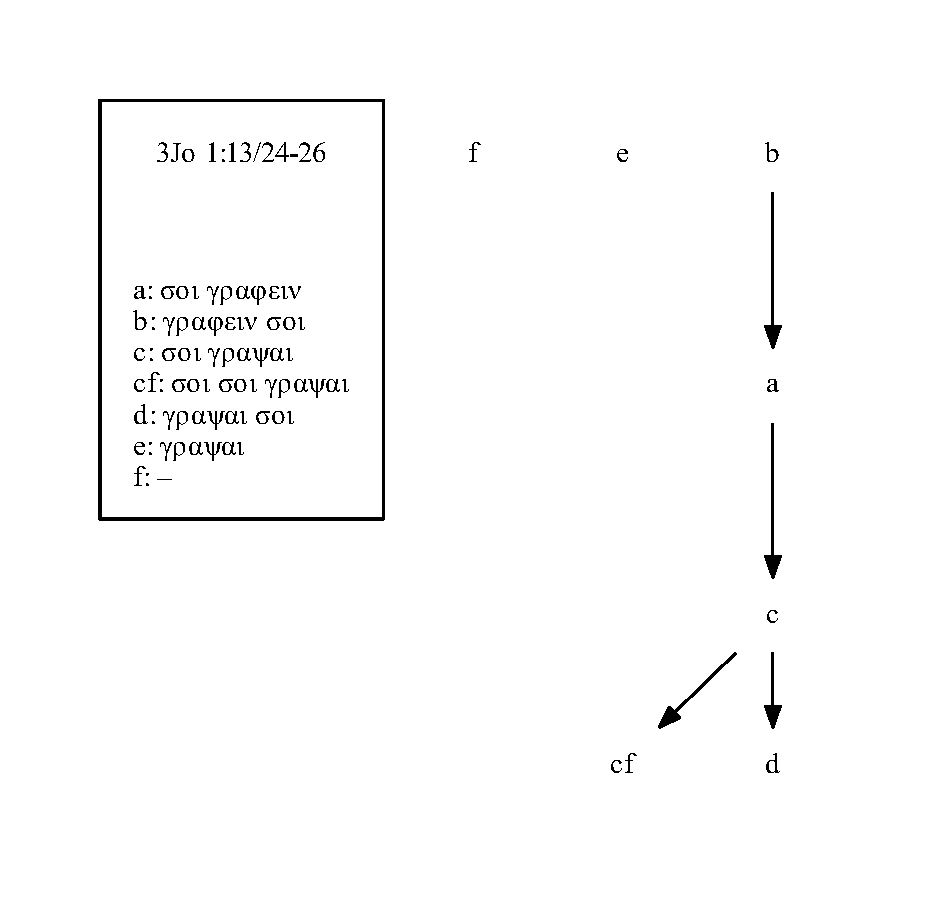
\includegraphics[width=\textwidth]{../img/B25K1V13U24-26-local-stemma-b-initial.pdf}
%			\end{column}
%		\end{columns}
%	\end{frame}
%	\begin{frame}
%		\begin{center}
%			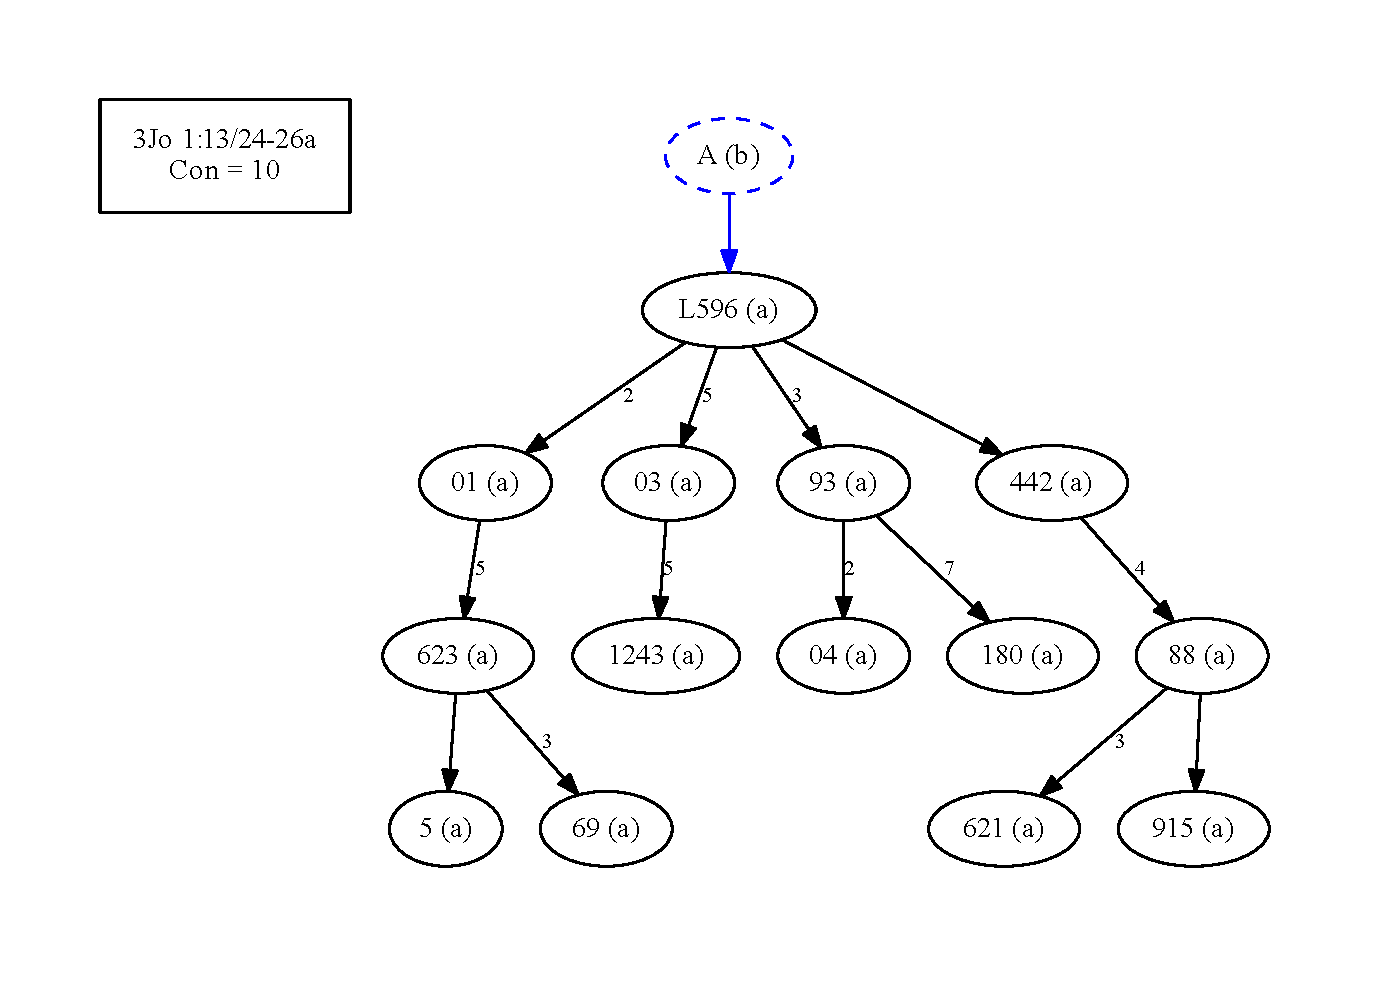
\includegraphics[width=\textwidth]{../img/B25K1V13U24-26Ra-coherence-attestations-b-initial.pdf}
%		\end{center}
%	\end{frame}
%	\begin{frame}
%		\begin{columns}
%			\begin{column}{0.45\textwidth}
%				\begin{itemize}
%					\item Or, we can look only at the parts of textual flow where a reading gets changed to find the most likely sources of unexplained readings (\emph{e} and \emph{f})
%				\end{itemize}
%			\end{column}
%			\begin{column}{0.45\textwidth}
%				\begin{center}
%					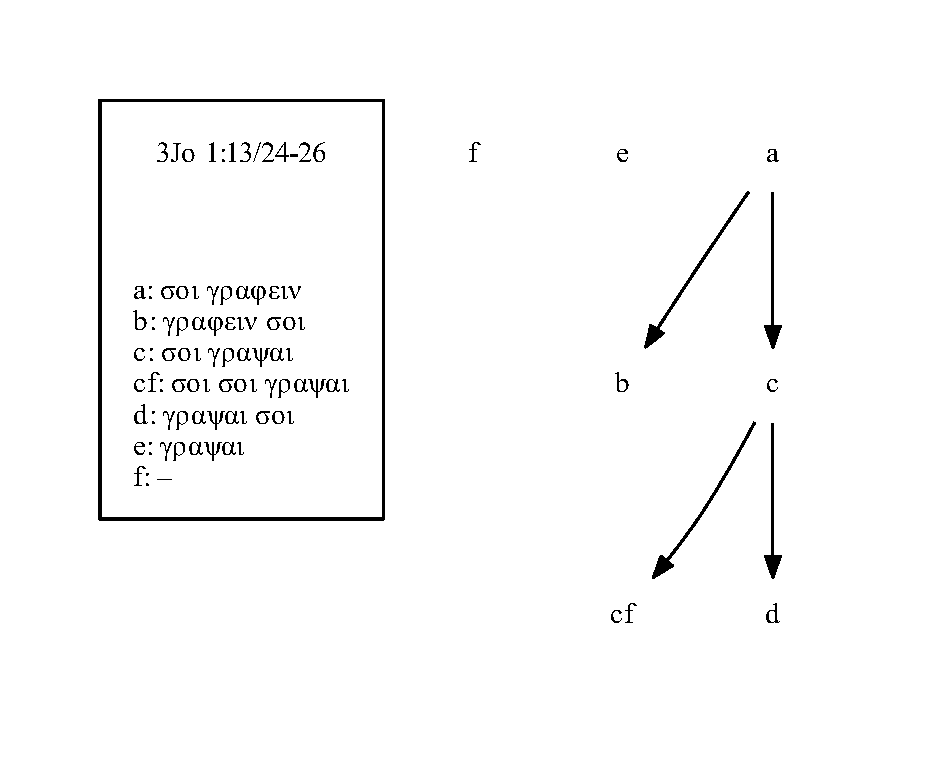
\includegraphics[width=\textwidth]{../img/B25K1V13U24-26-local-stemma-incomplete.pdf}
%				\end{center}
%			\end{column}
%		\end{columns}
%	\end{frame}
%	\begin{frame}
%		\begin{center}
%			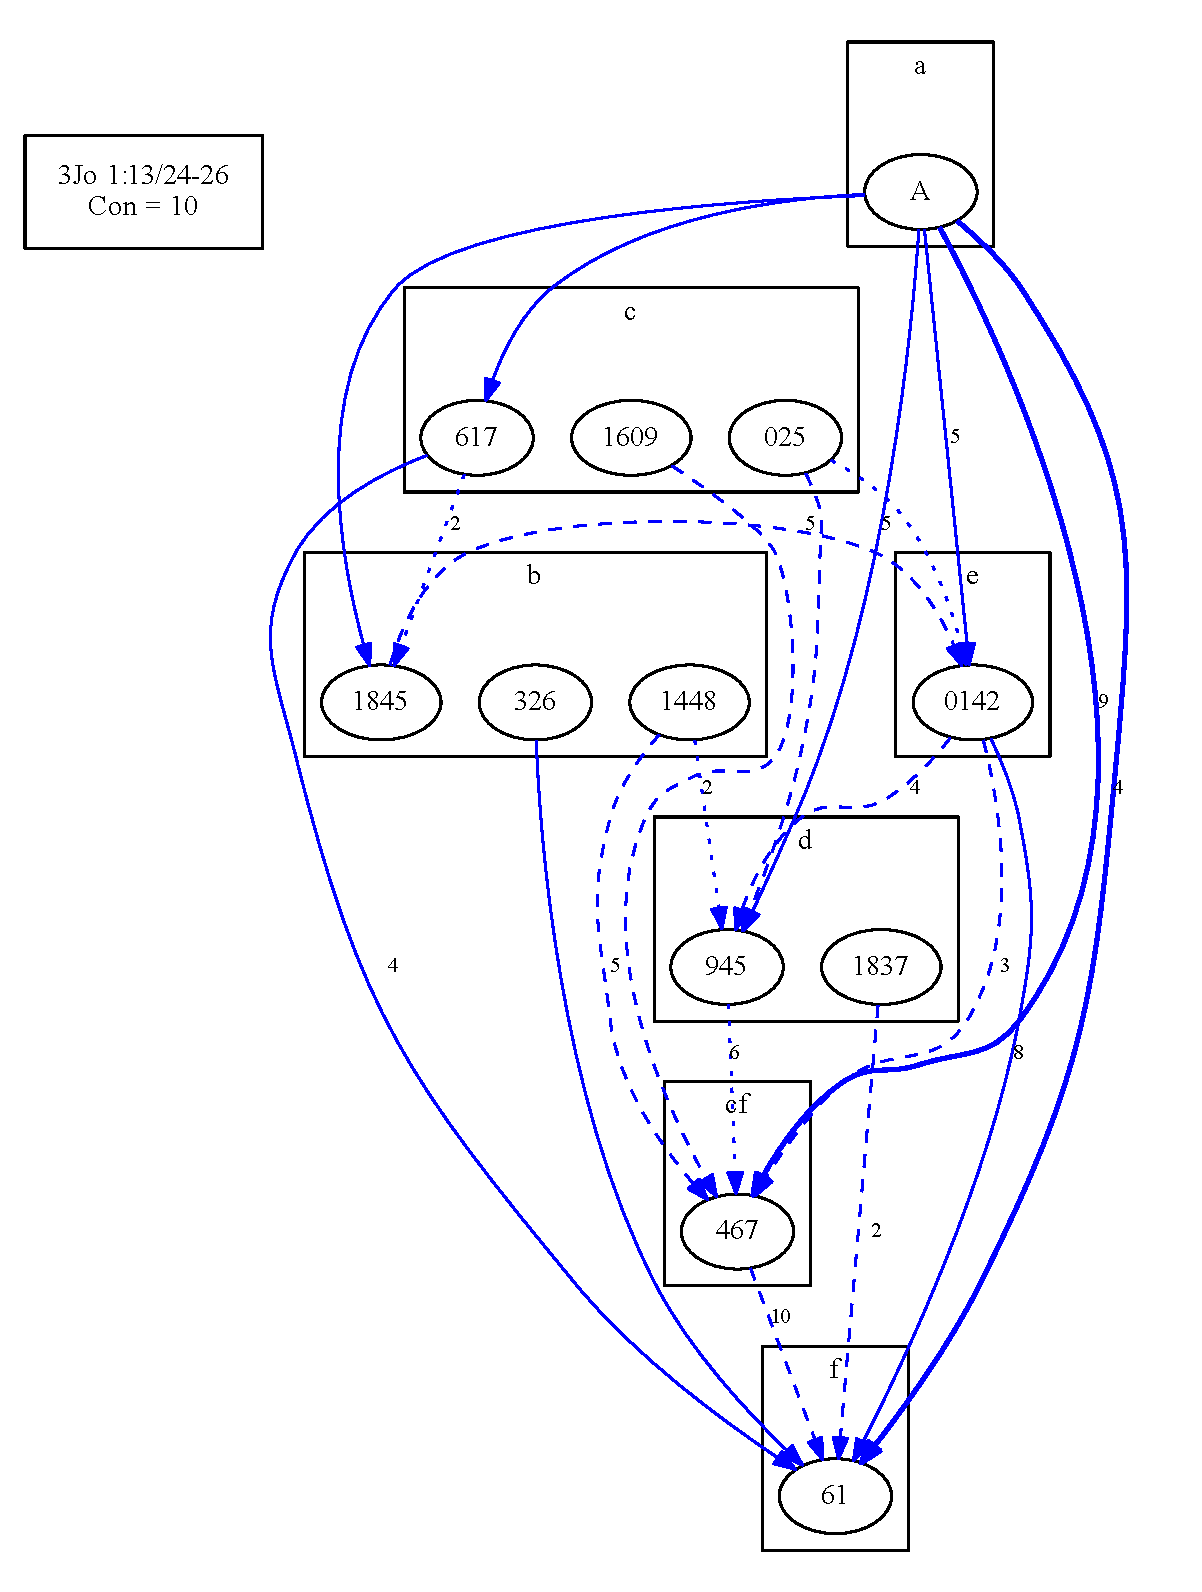
\includegraphics[width=0.5\textwidth]{../img/B25K1V13U24-26-coherence-variants-strengths.pdf}
%		\end{center}
%	\end{frame}
%	\begin{frame}{Textual Flow for a Variant Reading}
%		\begin{columns}
%			\begin{column}{0.45\textwidth}
%				\begin{itemize}
%					\item Using this information, we can attempt to explain previous unexplained readings
%					\item A necessary step for our ultimate goal of constructing a global stemma
%				\end{itemize}
%			\end{column}
%			\begin{column}{0.45\textwidth}
%				\begin{center}
%					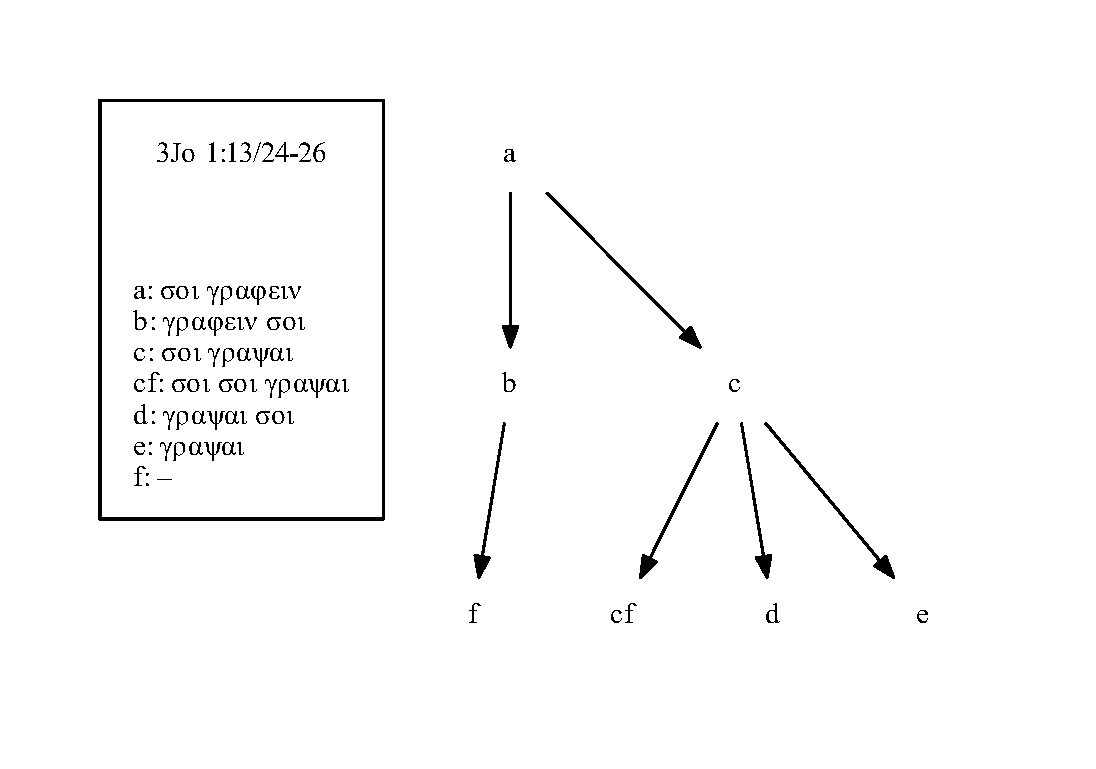
\includegraphics[width=\textwidth]{../img/B25K1V13U24-26-local-stemma-complete.pdf}
%				\end{center}
%			\end{column}
%		\end{columns}
%	\end{frame}
	\subsection{\textquote{Explained} Readings}
	\begin{frame}
		\begin{itemize}
			\item We say that one reading \emph{explains} another if
			\begin{itemize}
				\item it is the same reading (\textquote{explanation by agreement}), or
				\item there is an edge in the local stemma from it to the other reading (\textquote{explanation by descent})
			\end{itemize}
		\end{itemize}
		\begin{center}
			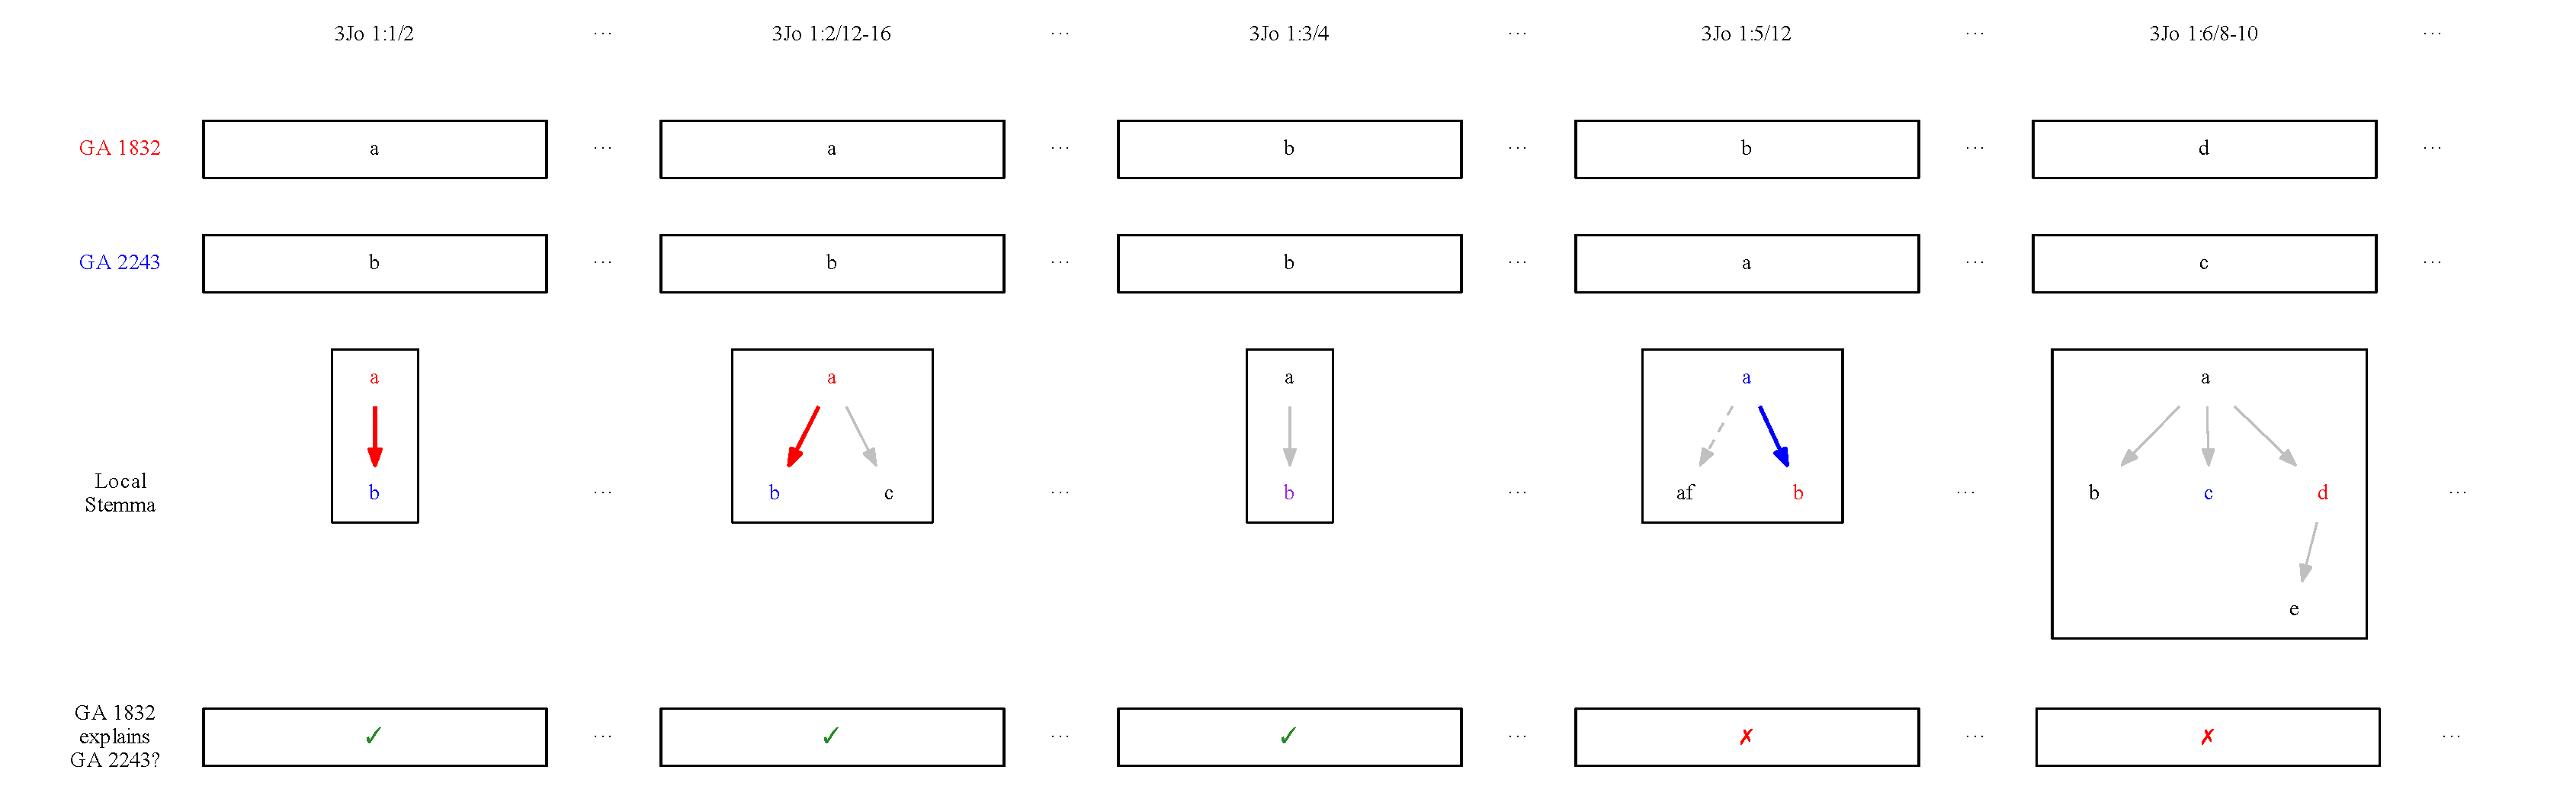
\includegraphics[width=\textwidth]{../img/explained-readings.pdf}
		\end{center}
		\begin{itemize}
			\item Lacunae do not have to be explained, and they cannot explain readings
		\end{itemize}
	\end{frame}
%	\begin{frame}
%		\begin{columns}
%			\begin{column}{0.4\textwidth}
%				\centering
%				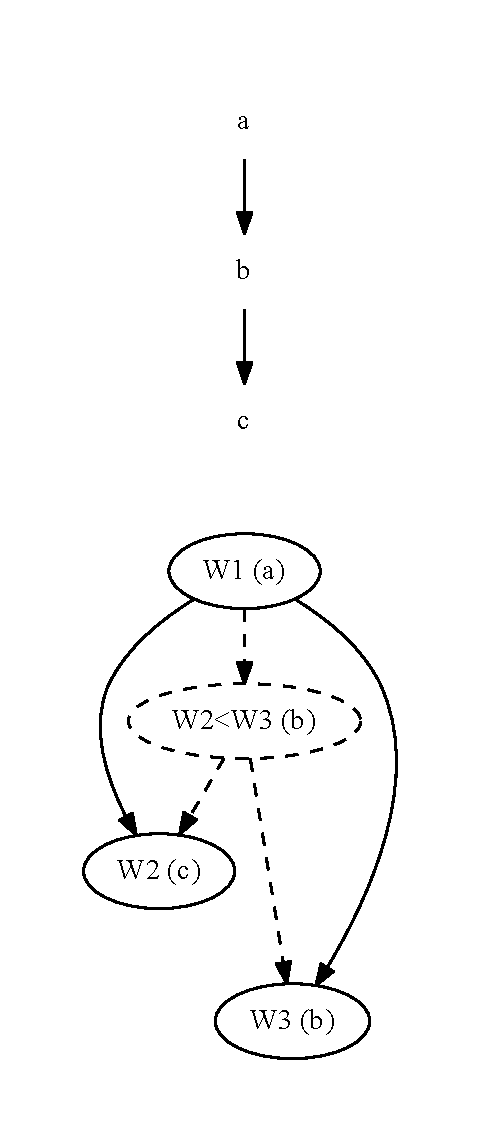
\includegraphics[width=0.75\textwidth]{../img/intermediary-node-example.pdf}
%			\end{column}
%			\begin{column}{0.55\textwidth}
%				\begin{itemize}
%					\item Does a reading explain any of its posterior readings transitively (i.e., in the local stemma to the left, does \emph{a} explain \emph{c})?
%					\item As originally formulated, \emph{no}: \emph{a} explains \emph{b} and \emph{b} explains \emph{c}, but \emph{a} does not explain \emph{c} (it's too many steps removed)
%					\item Later, in the global stemma, \emph{intermediary nodes} may be needed to ensure that all readings are explained
%				\end{itemize}
%			\end{column}
%		\end{columns}
%	\end{frame}
%	\begin{frame}
%		\begin{columns}
%			\begin{column}{0.4\textwidth}
%				\centering
%				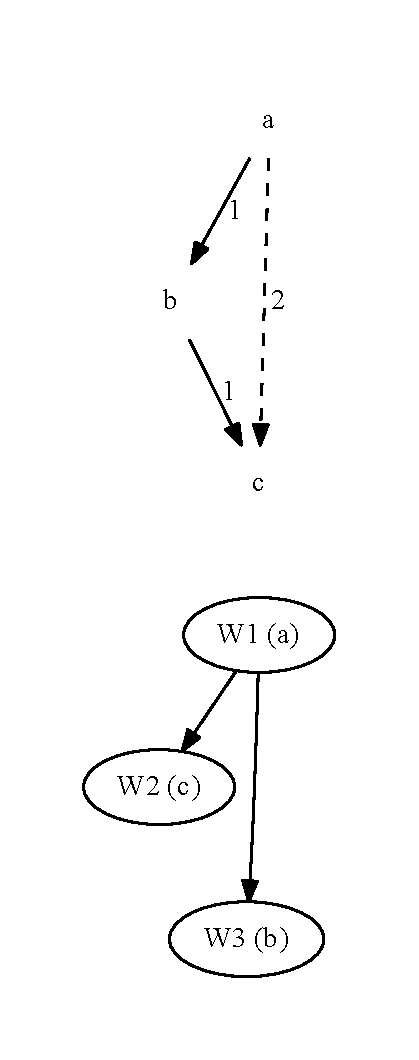
\includegraphics[width=0.75\textwidth]{../img/transitivity-example.pdf}
%			\end{column}
%			\begin{column}{0.55\textwidth}
%				\begin{itemize}
%					\item If we instead allow \emph{a} to explain \emph{c}, but at a higher cost (more on this in the substemma slides), then we remove the need for intermediary nodes (although multiple changes in the same variation unit may be implied along an edge in the global stemma)
%				\end{itemize}
%			\end{column}
%		\end{columns}
%	\end{frame}
	\subsection{Substemma(ta) of a Witness}
	\begin{frame}
		\begin{itemize}
			\item The \emph{substemma} of a witness is the portion of the global stemma consisting of the witness and its ancestors in the stemma
			\item Requirement: \emph{every} extant reading in the witness must be explained by a reading in at least one of its ancestors
		\end{itemize}
		\begin{center}
			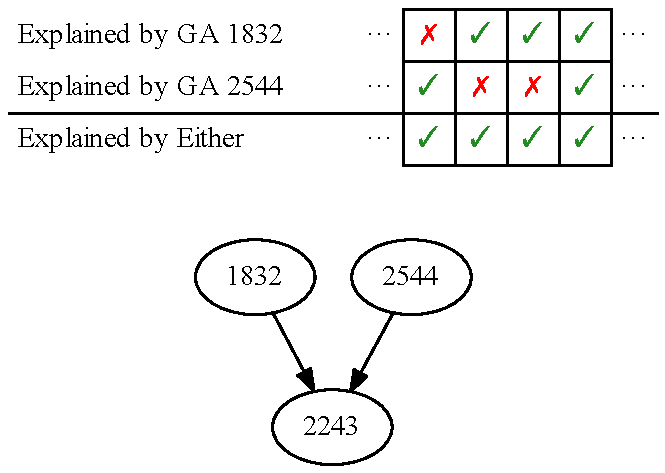
\includegraphics[scale=0.5]{../img/ga-2243-substemma.pdf}
		\end{center}
	\end{frame}
	\begin{frame}
		\begin{itemize}
			\item A witness may have multiple valid substemma (i.e., ones that explain all of its readings), but some are better than others
			\item Two of the CBGM's methodological assumptions are important here:
			\begin{enumerate}
				\setcounter{enumi}{2} % manually set the enumerate counter so that the first item is #3
				\item Scribes typically used fewer sources rather than many.
				\item Scribes typically used closely related sources rather than distant ones.
			\end{enumerate}
			\item Thus, we need a cost function to distinguish between candidate substemmata
		\end{itemize}
		\begin{center}
			\includegraphics[width=0.75\textwidth]{../img/substemmata.pdf}
		\end{center}
	\end{frame}
%	\begin{frame}
%		\begin{itemize}
%			\item Based on assumption 3, we should prefer substemmata with fewer ancestors (``parsimony'')
%			\item Based on assumption 4, we should prefer substemmata with ancestors that agree as often as possible with the witness
%			\item A balancing act: the substemma \{L938\} is more parsimonious, but may not explain as many readings by agreement
%		\end{itemize}
%		\begin{center}
%			\includegraphics[width=0.75\textwidth]{../img/substemmata.pdf}
%		\end{center}
%	\end{frame}
	\begin{frame}
		\begin{itemize}
			\item A simple cost function: \textquote{the number of variation units where the ancestor explains the witness by descent and not agreement}
			\item Thus, in the example below, GA 1832 is a stemmatic ancestor of 2243 with a cost of $2$ (but it cannot be its only stemmatic ancestor)
		\end{itemize}
		\begin{center}
			\includegraphics[width=\textwidth]{../img/explained-readings-costs.pdf}
		\end{center}
	\end{frame}
%	\begin{frame}
%		\begin{columns}
%			\begin{column}{0.45\textwidth}
%				\begin{itemize}
%					\item If we allow a reading to explain any reading posterior to it, then a better cost per variation unit is the length of the path from the prior reading to the posterior one.
%				\end{itemize}
%			\end{column}
%			\begin{column}{0.45\textwidth}
%				\begin{center}
%					\includegraphics[width=0.75\textwidth]{../img/transitivity-cost.pdf}
%				\end{center}
%			\end{column}
%		\end{columns}
%	\end{frame}
	\subsection{Substemma Optimization}
	\begin{frame}
		\begin{itemize}
			\item The process of finding the best substemma for a witness
			\item For $n$ potential ancestors, a \emph{weighted set cover} problem with $n$ sets 
			\item $2^n - 1$ possible combinations to check (!), but fast heuristics exist
		\end{itemize}
		\begin{center}
			\includegraphics[width=0.75\textwidth]{../img/weighted-set-cover.pdf}
		\end{center}
	\end{frame}
%	\begin{frame}
%		\begin{columns}
%			\begin{column}{0.4\textwidth}
%				\includegraphics[width=\textwidth]{../img/branch-and-bound-example.pdf}
%			\end{column}
%			\begin{column}{0.55\textwidth}
%				\begin{itemize}
%					\item If a witness has many potential ancestors, then checking all $2^n - 1$ possible substemmata by brute force is prohibitive
%					\item The \emph{branch-and-bound} heuristic (pictured left) finds all minimum-cost substemmata quickly in practice
%					\item Easily adapted to find all substemmata within a given cost
%				\end{itemize}
%			\end{column}
%		\end{columns}
%	\end{frame}
	\subsection{Global Stemma}
	\begin{frame}
		\begin{columns}
			\begin{column}{0.45\textwidth}
				\begin{itemize}
					\item Just as the local stemma relates readings, the \emph{global stemma} relates witnesses
					\item Combination of all substemmata into a single graph
					\item Analogous to a phylogenetic stemma
				\end{itemize}
			\end{column}
			\begin{column}{0.45\textwidth}
				\begin{center}
					\includegraphics[width=\textwidth]{../img/partial-global-stemma.pdf}
				\end{center}
			\end{column}
		\end{columns}
	\end{frame}
%	\begin{frame}
%		\begin{columns}
%			\begin{column}{0.45\textwidth}
%				\begin{itemize}
%					\item But \emph{every reading in every local stemma} except the initial one must be explained by another reading
%					\item Otherwise…
%				\end{itemize}
%			\end{column}
%			\begin{column}{0.45\textwidth}
%				\begin{center}
%					\includegraphics[width=0.875\textwidth]{../img/B25K1V13U24-26-local-stemma-incomplete.pdf}
%				\end{center}	
%			\end{column}
%		\end{columns}
%		\begin{center}
%			\includegraphics[width=\textwidth]{../img/global-stemma-incomplete.pdf}
%		\end{center}	
%	\end{frame}
	\begin{frame}
		\begin{itemize}
			\item How does this differ from a phylogenetic stemma?
			\begin{itemize}
				\item Converging branches (reflecting contamination) are allowed
				\item In practice, it takes much less time to produce a global stemma (minutes) than it does to do a satisfactory phylogenetic search for promising stemmata (> a day)
				\item No hyparchetypes, and texts found in later manuscripts can be ancestors to texts found in earlier manuscripts
				\item Can it model a history of the text?
			\end{itemize}
		\end{itemize}
		\begin{center}
			\includegraphics[width=\textwidth]{../img/global-stemma-complete.pdf}
		\end{center}	
	\end{frame}
	\section{Conclusions}
	\sectionframe
	\begin{frame}
		\begin{itemize}
			\item Can we get the advantages of both approaches?
			\item The CBGM could use cost graphs instead of local stemmata
			\item Phylogenetics could use the \emph{local-genealogical principle} to model contamination
			\begin{itemize}
				\item Different low-cost stemmata at different variation units
			\end{itemize}
		\end{itemize}
		\begin{center}
			\begin{columns}
				\begin{column}{0.3\textwidth}
					\centering
					\includegraphics[scale=0.25]{../img/gene-tree-rooted-site-1.pdf}\\
					\vspace{\baselineskip}
					\includegraphics[scale=0.25]{../img/gene-tree-rooted-site-2.pdf}
				\end{column}
				\begin{column}{0.1\textwidth}
					\centering
					$\Rightarrow$
				\end{column}
				\begin{column}{0.5\textwidth}
					\centering
					\includegraphics[scale=0.5]{../img/stemma-rooted-contamination.pdf}
				\end{column}
			\end{columns}
		\end{center}
	\end{frame}
%	\begin{frame}{Criticisms and Idiosyncrasies}
%		\begin{itemize}
%			\item Biggest idiosyncrasy: \emph{no reconstruction of hypothetical ancestors} (because contamination is assumed to make this impossible)
%			\begin{itemize}
%				\item (Personal opinion: this assumption is made for practical rather than theoretical reasons)
%				\item Texts of extant witnesses = bad representatives of ancestors of other extant texts
%				\item CBGM may see ``contamination'' where there's just a gap in the textual tradition
%				\item Enough of the tradition is lost to make this a problem
%			\end{itemize}
%			\item Can the global stemma be understood as a history of the text?
%		\end{itemize}
%	\end{frame}
%	\begin{frame}{Criticisms and Idiosyncrasies}
%		\begin{itemize}
%			\item Recommended reading:
%			\begin{itemize}
%				\item \cite{Jongkind14}
%				\item The special feature articles in \emph{TC} 20 (2015)
%				\item \cite{Gurry18}
%				\item \cite{Carlson20} (but see \href{http://ntvmr.uni-muenster.de/en_US/intfblog/-/blogs/remarks-on-carlson-a-bias-at-the-heart-of-the-cbgm-guest-post-by-gerd-mink-}{Mink's response})
%			\end{itemize}
%		\end{itemize}
%	\end{frame}
	\section{Questions?}
	\sectionframe
\end{document}